\part{Modélisation du théâtre d’Orange}

	\chapter*{Introduction}
	\addcontentsline{toc}{chapter}{Introduction}
	
			 Le théâtre antique d'Orange situé dans le Vaucluse est le théâtre romain le mieux conservé d'Europe et un des trois seul au monde a avoir conservé son mur de scène. Il est adossé à la colline Saint-Eutrope sur laquelle sa \gls{cavea} repose partiellement.
			 
			 En 45 avant notre ère, suite à la victoire de César sur la Gaulle, de larges vagues de colonisation amenèrent des soldats vétérans à s'installer dans la province de Gaule transalpine qu'August réorganise par la suite en province de Narbonnaise. L'architecture urbaine est alors régie par les écrits de \cite{vitruve} et de nombreux théâtres sont construit comme celui d'Arles en 20 avant notre ère. La construction du théâtre de Aurosio (l'ancienne ville d'Orange) fut démarrée par les vétérans de la II\up{e} légion gallique de César vers 10 avant notre ère et dura quelques dizaines d'années. \citep{PouvoirDuTheatre} Cette origine nous est d'ailleurs rappelée par la présence du sigle C.I.S (\textit{Colonia Iulia Secundanorum}) inscrit à plusieurs endroit du grand mur du \gls{postscaenium} \cite{formige}. 
			 
			 Lorsque le théâtre fut abandonné comme édifice de spectacle, il ne fut pas détruit. Les princes d'Orange y firent installer un poste avancé de leur château et l’ensemble de l’édifice fut investi par des habitations utilisant le mur de scène comme rempart de protection (fig. \ref{av_deblaiement}). Au XVII\up{e} siècle le roi Louis XIV qualifiait en ces mots son impressionnant mur de scène de 103m de large par 37m de haut comme : « La plus belle muraille de mon royaume » et quelques écrits tentèrent d'imaginer les démonstrations qui pouvaient se tenir dans ce lieu de spectacle. 
			 
			 Ce n'est pourtant qu'au XIX\up{e} siècle que débuta un vaste chantier de déblaiement de l'enceinte dans le but de restituer au bâtiment son rôle premier. Avec ce projet apparurent les premières images d'archive du théâtre. En charge du chantier, Augustin Caristie fait paraitre en 1846, \textit{"Monuments antiques à Orange, arc triomphe et théâtre"} oeuvre de référence qui recense l'état des vestiges avant et après la destruction des maisons. Ces textes et dessins bien que, comme le stipule l'auteur, parfois hypothétiques sont par la suite complétés par d'autres architectes comme Pierre-Honoré Daumet qui réalisa en 1873 le relevé des élévations du monument. Les premières représentations théâtrales modernes purent alors avoir lieu. \`{A} la fin du siècle l'architecte Jean-Camille Formigé fut chargé de restaurer la \gls{cavea} selon les indications de Caristie et en s'inspirant du modele de Vitruve. Son fils Jules Formigé poursuivit son travail et mis à jour de nombreux éléments de décors notamment en creusant au niveau de l'\gls{hyposcaenium}. Depuis les années 20 jusqu'aux années 80 de nombreuse restaurations ou constructions ont été effectués avec une rigueur archéologique contestable dans le but principalement d'habiller le lieu plus que pour le restituer. En 1981 le théâtre entre au patrimoine mondiale de l'UNESCO et quelques années plus tard d'autres constructions modernes tels que la couverture métallique de la scène viennent s'ajouter, détériorant au passage une partie de la maçonnerie antique. Certains projets ont pu être stoppés avant que des dégâts irréparables ne soient créer comme la créations d'ascenseurs dans le mur de scène. Malgré tout, ces travaux ont souvent été entrepris sans le moindre regard archéologique et de nombreuses données ont été perdues \citep{carteArcheo}.
			 
			 Depuis la fin du XX\up{e} siècle l'\gls{iraa} a relancé une étude approfondie du bâtiment et de sa décoration avec une approche archéologique rigoureuse. C'est dans cette démarche que cette thèse s'interface avec pour objectif la modélisation numérique du théâtre. Dans cette première partie nous allons donc présenter l'agencement architectural du bâtiment sans entrer dans les détails de sa décoration. Nous détaillerons ensuite les méthodes de modélisation graphique utilisées et finirons par exposer les nouveaux éléments archéologiques découlant de ce travail.
			 
		
\begin{figureth}
	\begin{subfigureth}{0.49\textwidth}
		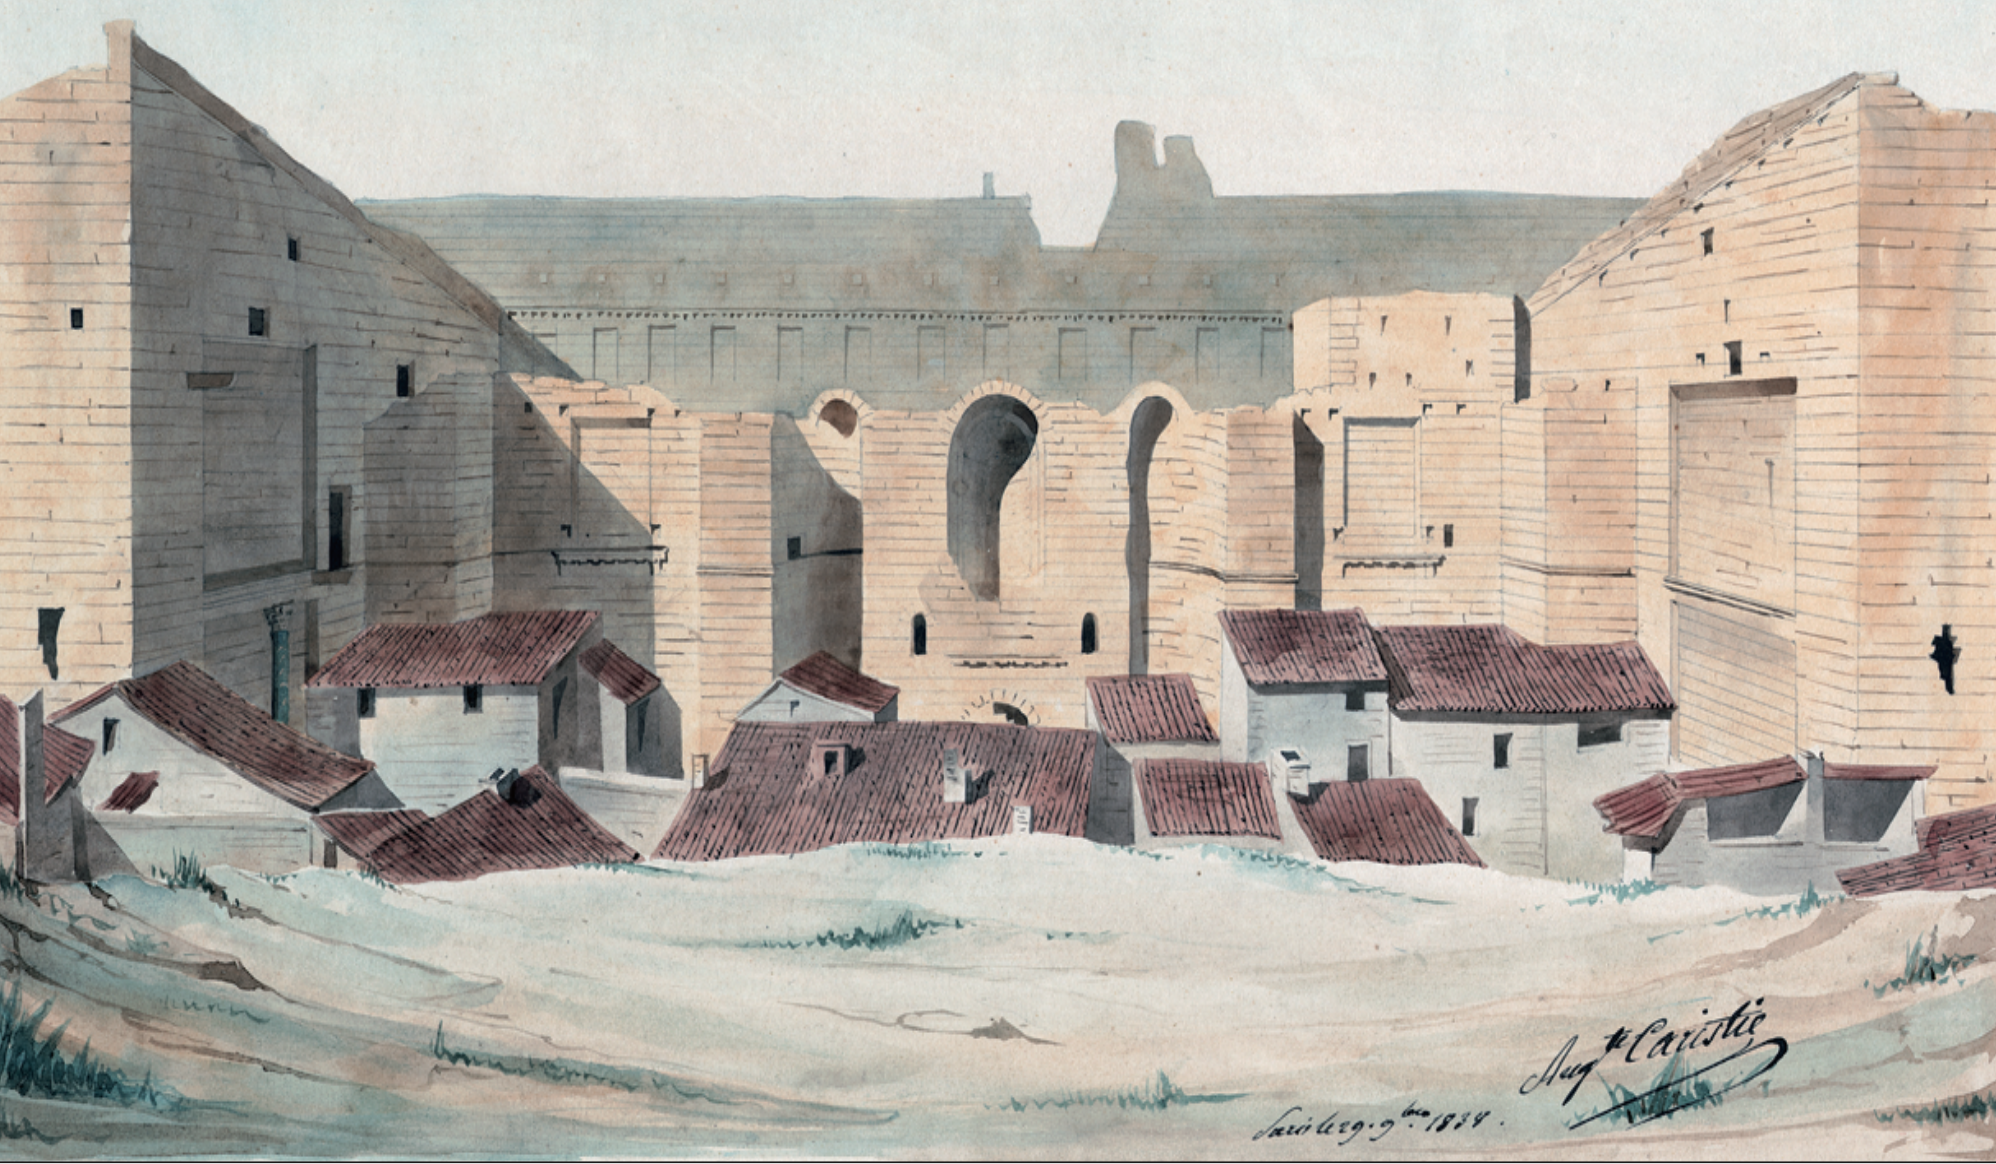
\includegraphics[width=\linewidth]{images/av_deblaiement}
		\caption{Vue de la scène avant le déblaiement par A. Caristie, 1856 (cliché Médiathèque de l’Architecture et du Patrimoine, Charenton)}
		\label{av_deblaiement}
	\end{subfigureth}
	\begin{subfigureth}{0.47\textwidth}
		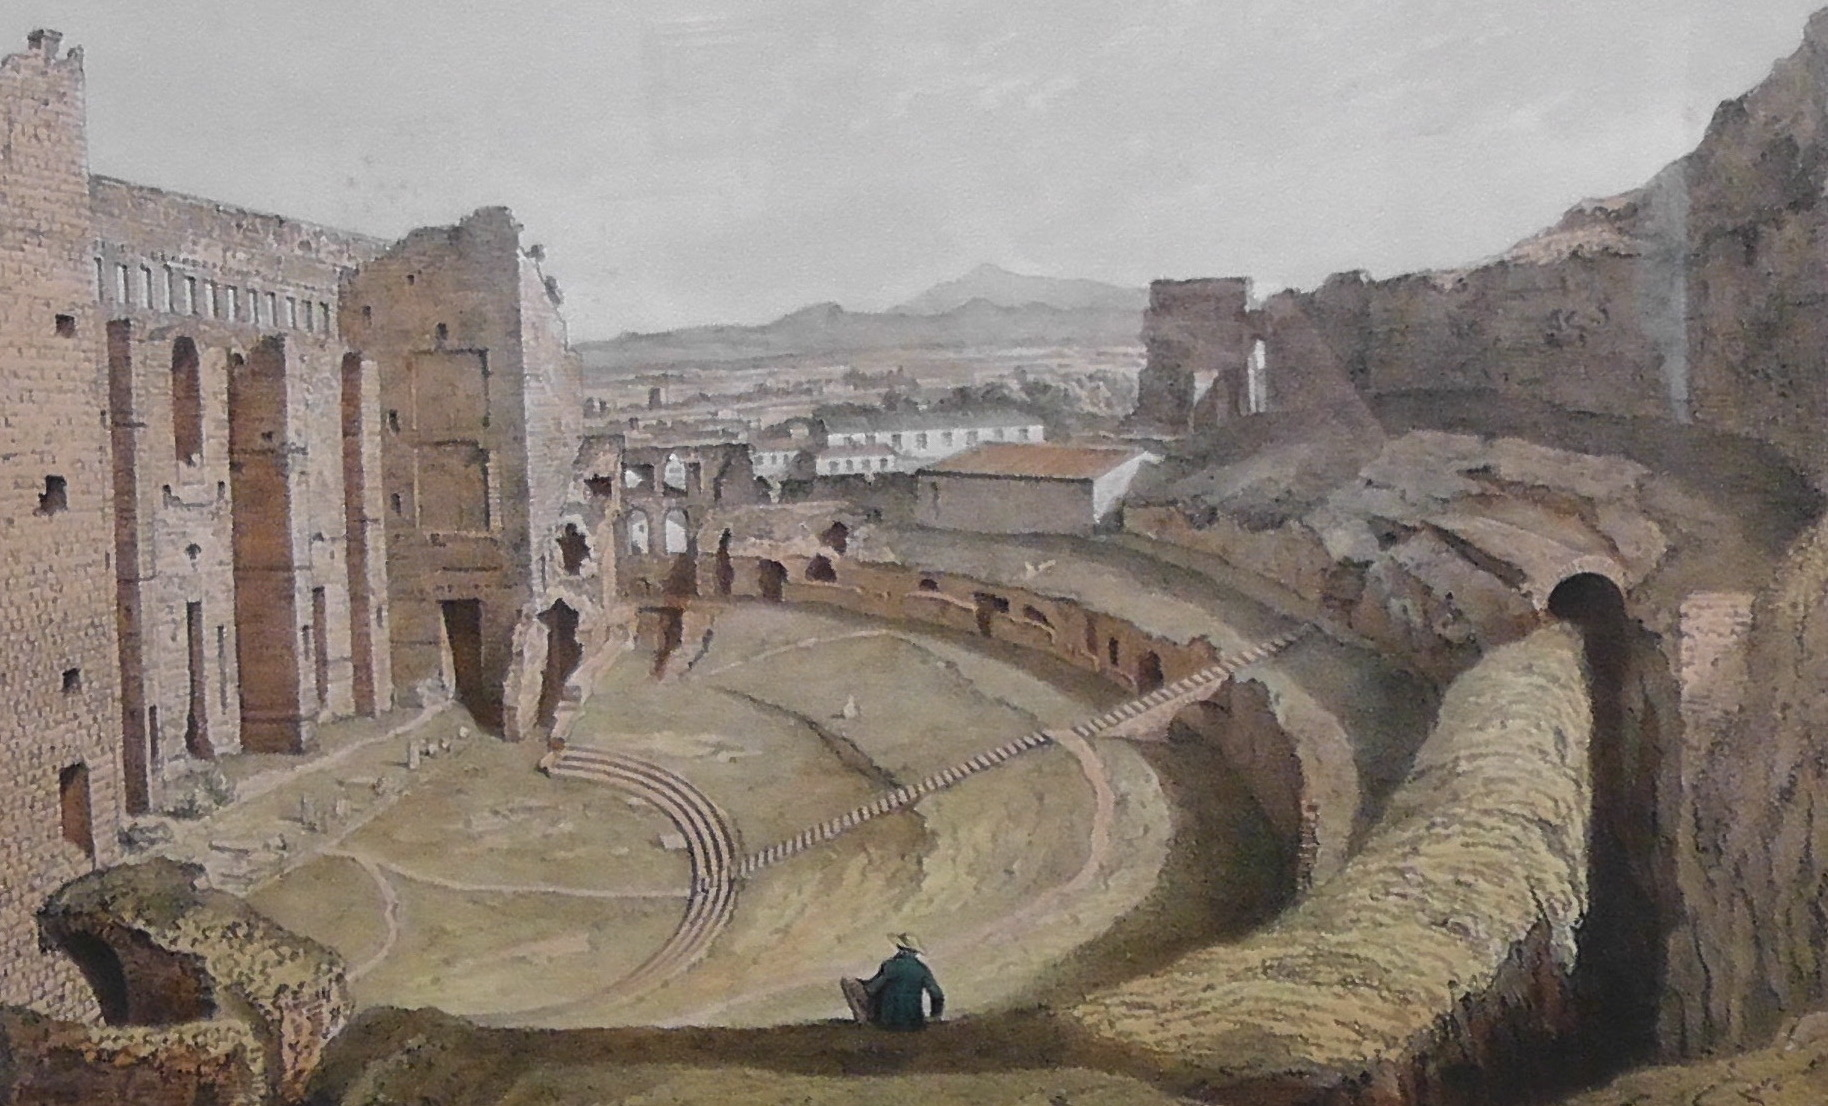
\includegraphics[width=\linewidth]{images/asselineau}
		\caption{Vue intérieure du théâtre, par Asselineau, XIX\up{e} siècle, Musée d'Art et d'Histoire d'Orange}
	\end{subfigureth}
	\caption[Théâtre d'Orange avant restauration]{Dessins du théâtre d'Orange avant et après déblaiement par A.Caristie}		
	%\label{fig:caristie}
\end{figureth}		

		
	\chapter{Architecture générale du théâtre d'Orange}
		\citationChap{
		L'architecture, c'est ce qui fait les belles ruines
		}{Auguste Perret}
		\minitoc
		\newpage
		
		\section{Introduction}
		
		En 2013, l'\gls{iraa} lance une série de campagnes de mesure et d'analyse du théâtre d'Orange d'une part grâce à des relevés effectués sur le terrain et d'autre part à l'aide d'une étude approfondie des documents d'archive conservés pour la plupart à la Médiathèque de l'architecture et du patrimoine à Charenton-le-Pont. Ceux-ci comportent les plans de Caristie et Daumet et permettent d'avoir une vision du théâtre avant que celui-ci ne soit restauré par Formigé. L'étude réalisée durant cette thèse est donc principalement basée sur le rapport de l'\gls{iraa} résultant de ces travaux d'analyse : \cite{orangeTxt} et \citep{orangePl}.
		
		Le théâtre d'Orange a été bâtie en partie selon les indications de \cite{vitruve} et suit donc les préceptes de l'architecture romaine de l'époque impériale. Comme la plupart de ces édifices, il se présente en demi-cercle fermé par un mur rectiligne. Sa \gls{cavea} tournée vers le Nord est adossée à la colline Saint-Eutrope offrant ainsi un support naturel à l'édifice. A la différence des \glspl{odeon} seul un \gls{velum} servait de toiture aux spectateurs. Collé au flan est au théâtre se trouvent les ruines d'un sanctuaire du culte impérial qui ne fait pas partie de l'étude. 

\begin{figureth}
		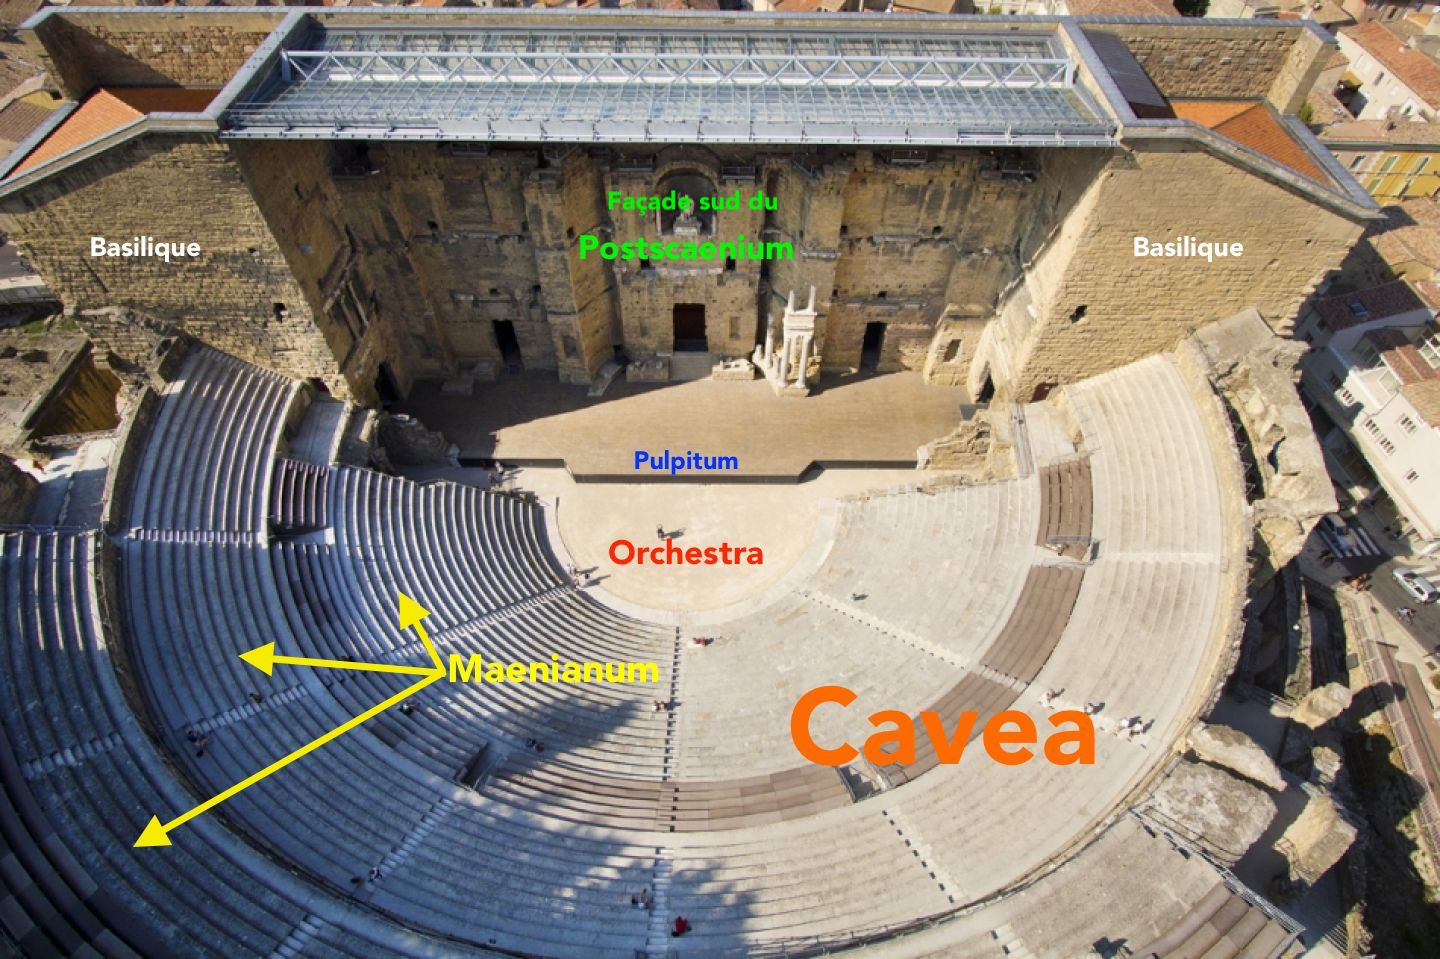
\includegraphics[width=\linewidth]{images/vuensemble}
		\caption[Vue d'ensemble du théâtre d'Orange]{Vue d'ensemble du théâtre d'Orange (cliché de Boudereaux sur choregies.fr)}
\end{figureth}


		\section{Le \gls{postscaenium}, les \glspl{basilique} et le \gls{pulpitum}}
		
		Le \gls{postscaenium} (ou mur de scène) constituant la façade nord du bâtiment ainsi que les deux \glspl{basilique} l'enclavant constituent les parties les mieux conservées du théâtre. Le \gls{postscaenium} servait de décor pour les représentations et tenait probablement un rôle acoustique (voir \Nameref{part3}). Les côtés est et ouest donnaient sur des rues, alors qu'adossé à la façade nord se trouvait une \gls{porticus ps} large d'environ neuf mètres. Celle-ci se trouvant à l'extérieur du théâtre, elle ne fera pas partie de l'étude. Elle donne néanmoins accès au \gls{postscaenium} par le biais de dix-sept portes reparties de manière symétrique par rapport à la porte centrale. Sur la partie haute de la façade se trouve deux séries de \glspl{console} ainsi qu'une assise de bouches d'eau qui permettaient d'évacuer les eaux qui tombaient sur le toit du bâtiment de scène. Les \glspl{console} de la série supérieure (mis à part les deux situées aux extrémités) présentent un trou traversant permettant d'accueillir le mât. Celles de la série inférieure sont creusées à leur lit d'attente d'une grande mortaise circulaire prolongée par un petit trou permettant l'écoulement de l'eau de pluie. Pour pouvoir placer un mât dans un couple \glspl{console} il fallait également que l'assise de bouche d'eau soit percée. Or cela n'est le cas que pour douze emplacements correspondant aux mâts n\no4 à 9 à partir des deux extrémités du mur. Il semble que les mâts n'aient été présents qu'à ces emplacements, c'est à dire au niveau des \glspl{basilique} et non du mur de scène pour soulager ce dernier d'une trop forte tension liée au poids du \gls{velum}. Néanmoins, il est aussi possible de supposer que les \glspl{console} aient été initialement prévues pour couvrir l'estrade par des voiles montées sur des vergues comme à Aspendos et que l'idée fut abandonnée en cours de construction au profit d'une toiture de tuiles sur charpente de bois \cite{moretti}. L'intérieur du \gls{postscaenium} comporte huit pièces donnant uniquement sur la \gls{porticus ps} à l'extérieur du théâtre. Ces pièces servaient de coulisse l'habillement des acteurs ou le stockage des décors et costumes. Trois portes, dont la porte royale, donnent directement accès à la scène. Deux portes de part et d'autre amène aux \glspl{basilique} et une au \gls{parascaenium} et à des escaliers permettant de monter aux étages supérieurs. \`{A} l'intérieur du \gls{postscaenium}, en plus du rez-de-chaussé et des combles, on compte deux étages assurés par la présence de baies à arcature permettant de passer d'une pièce à l'autre à l'intérieur du mur. Cela permettait aux acteurs d'accéder à des niches traversante en hauteur pour faire apparaitre par exemple des personnages divins ou effectuer des bruits de tonnerre. 
		
		La façade sud du mur (ou front de scène) est celle qui servait de décor aux spectacles. Aujourd'hui, il ne reste que le mur en calcaire de Courthézon (calcaire de couleur jaune foncé-beige) qui été jadis caché par des ornementations en marbre. On y trouve plusieurs niches de diverse profondeurs ainsi que les traces d'encastrement du placage de marbre qui servent de repère aux archéologues pour reconstituer la décoration. Le mur a une géométrie symétrique par rapport à l'axe décrit par la porte royale rectangulaire et la niche voutée située au dessus et accueillant aujourd'hui une statue dite "d'Auguste" (faite de ciment et de fragments antiques et placée là en guise de décoration en 1944). Cet axe est placé sur une paroi rectiligne qui fait saillie au fond d'une \gls{exedre} curviligne ce qui donne un effet de "focus" vers la porte royale et la niche voutée. De part et d'autre se trouvent deux  \glspl{exedre} rectangulaires peu profondes. Le mur est découpé verticalement en trois ordres sur les extrémités et seulement deux sur la partie centrale. Au dessus se trouve l'espace réservé au toit qui couvrait le \gls{postscaenium} et la scène. On y voit aujourd'hui les trous d'encastrement dans lesquelles venaient s'insérer les poutres.
		
		Le mur de façade du bâtiment de scène est flanqué de part et d'autres de deux \glspl{basilique} de forme presque carrée auxquelles on accède depuis la scène par une grande porte rectangulaire et un \gls{parascaenium}. Celui-ci comporte un escalier permettant d'atteindre les niveaux supérieurs du \gls{postscaenium}. Les \glspl{basilique} sont composées de deux niveaux séparés par un toit en bois et accessible que depuis le rez-de-chaussée. On retrouve cela dans les théâtres d'Arles, Aspendos ou de Marcellus à Rome par exemple. Leur taille monumentale semble indiquer une fonction de foyer luxueux permettant aux spectateurs de se retrouver pendant les entre-actes ou en cas d'intempéries. Elles pouvaient également servir de coulisse pendant les spectacles ou pour stocker les éléments de décor volumineux. Ces salles étaient accessibles par les trois cotés autres que la scène par un couple de baies à arcature. Une baie à arcature donne également sur le postscaenium qui s'ouvre dans le même alignement sur la scène via une porte rectangulaire.
		
		La scène ou \gls{pulpitum} était une structure en bois d'une largeur de 61m et d'une profondeur de 10m et a complètement disparu. Elle était ornée en sa devanture par une décoration de marbre souvent composée de niches rondes ou carrées alternées. Vitruve dit que sa hauteur ne doit pas excéder cinq pieds (soit 1m50) afin que les spectateurs assis dans l'orchestre voient facilement. Celle de Orange s'élève à 1m20 d'après les traces laissées sur le mur de scène. En dessous se trouve l'hyposcaenium qui étaient composé principalement d'une fosse et d'un espace dédié à la machinerie du rideau de scène. Effectivement, entre le mur de front du \gls{pulpitum} et la scène, un rideau en étoffe peinte ou tissée d'une hauteur de moins de trois mètres descendait pour laisser apparaitre la scène aux spectateurs. Il venait s'enrouler autour de cylindres et était actionné par un système de poulies et contrepoids. Une fois descendu, le plancher venait se refermer au dessus de cet espace permettant ainsi aux acteurs de s'approcher jusqu'au bord du \gls{pulpitum}, voire de descendre au niveau de l'\gls{orchestra}. Le plancher était soutenu par des poutres et les acteurs ou les machinistes pouvaient se rendre en dessous par le biais de trappe et d'escaliers. Le mur de décoration est par ailleurs bordé par un caniveau afin d'évacuer les eaux de pluie.
						
		\section{L'\gls{orchestra}, les \gls{aditus} et la \gls{cavea}}
		
	
	L'\gls{orchestra} est la partie semi-circulaire situé entre la scène et le premier gradin. Anciennement nommée "choros", chez les grecs qu'elle y accueillait le choeur, elle ne sert plus aux représentations chez les romains et certains spectateur de marque pouvaient s'y installer. Aujourd'hui recouverte de graviers compact elle pouvait être à l'époque dallée de marbre ou pavé de pierres colorées. L'\gls{orchestra} était limité par un \gls{balteus} qui marquait la séparation avec la \gls{cavea} et qui surplombait un petit caniveau permettant d'évacuer l'eau de pluie. Elle comportait aussi des escaliers qui pouvaient mener à la scène soit pas le centre soit par les extremités \citep[p. 52]{formige}.
	
Depuis l'extérieur du théâtre on accède à ce lieu par deux larges \gls{parodos} formant les \gls{aditus}. Chacune est composée d'une succession de trois voûtes en décrochement qui portaient les extrémités de la \gls{cavea} et les tribunes. Celles-ci, considérées comme des places d'honneur étaient souvent décorées de sculpture comme à Dougga ou à Herculanum et étaient accessible par des escaliers particuliers. Ces entrées étaient dallées sur toute leur longueur mais sont aujourd'hui recouvertes par un sol moderne \cite[Pl. XVI]{orangePl}.
	
		La  \gls{cavea}, telle qu'elle a été restaurée, comprend trois hémicycles appelés \gls{maenianum}, séparée l'un de l'autre par une \gls{precinction} et un \gls{podium}. Cela a été déduit par Caristie de par le profil des \gls{aditus} et les vestiges des substructures et fut reconstruit en ce sens par Formigé. Chaque \gls{maenianum} est divisé en un certains nombre de sections appelées \gls{cuneus} par des escaliers. La forme de la \gls{cavea} ne suit donc pas les tracés de \cite{vitruve} de demi-cercle exacte mais présente plutôt une forme de fer à cheval.
		
		
Le premier \gls{maenianum}, ou \textit{ima cavea} est séparé par cinq escaliers en quatre \gls{cuneus} comme le révèle les vestiges des premiers gradins dégagé pendant les fouilles. Il comprend un repose-pied à sa base et vingt gradins comme à Aspendos, à Athènes (odéon d'Hérode Atticus) ou à Pompéi (grand théâtre). Leur hauteur moyenne est de 40cm et leur largeur de 80cm \cite{formige}. Au niveau de la première \gls{precinction} neuf ouvertures donnent  sur un couloir souterrain (premier \gls{ambulacre}). Ce dernier est accessible depuis l'extérieur du théâtre au rez-de-chaussée par deux escaliers longeant les \gls{aditus}. Le couloir ouvre aussi sur dix-huit pièces aveugles, mais seules les salles numérotées de 1 à 8 (fig. \ref{1erniveau}) sont des constructions antiques. Il était également possible de rejoindre le premier \gls{maenianum} à mi-hauteur depuis les \gls{parodos} par le biais de deux escaliers installés sous les gradins. Ceux-ci n'ont pas été remis en fonction lors de la restauration. Les \gls{vomitorium} et les \glspl{precinction} étaient généralement bordés de balustrades souvent ornées de sculptures.
		
	\begin{figureth}
		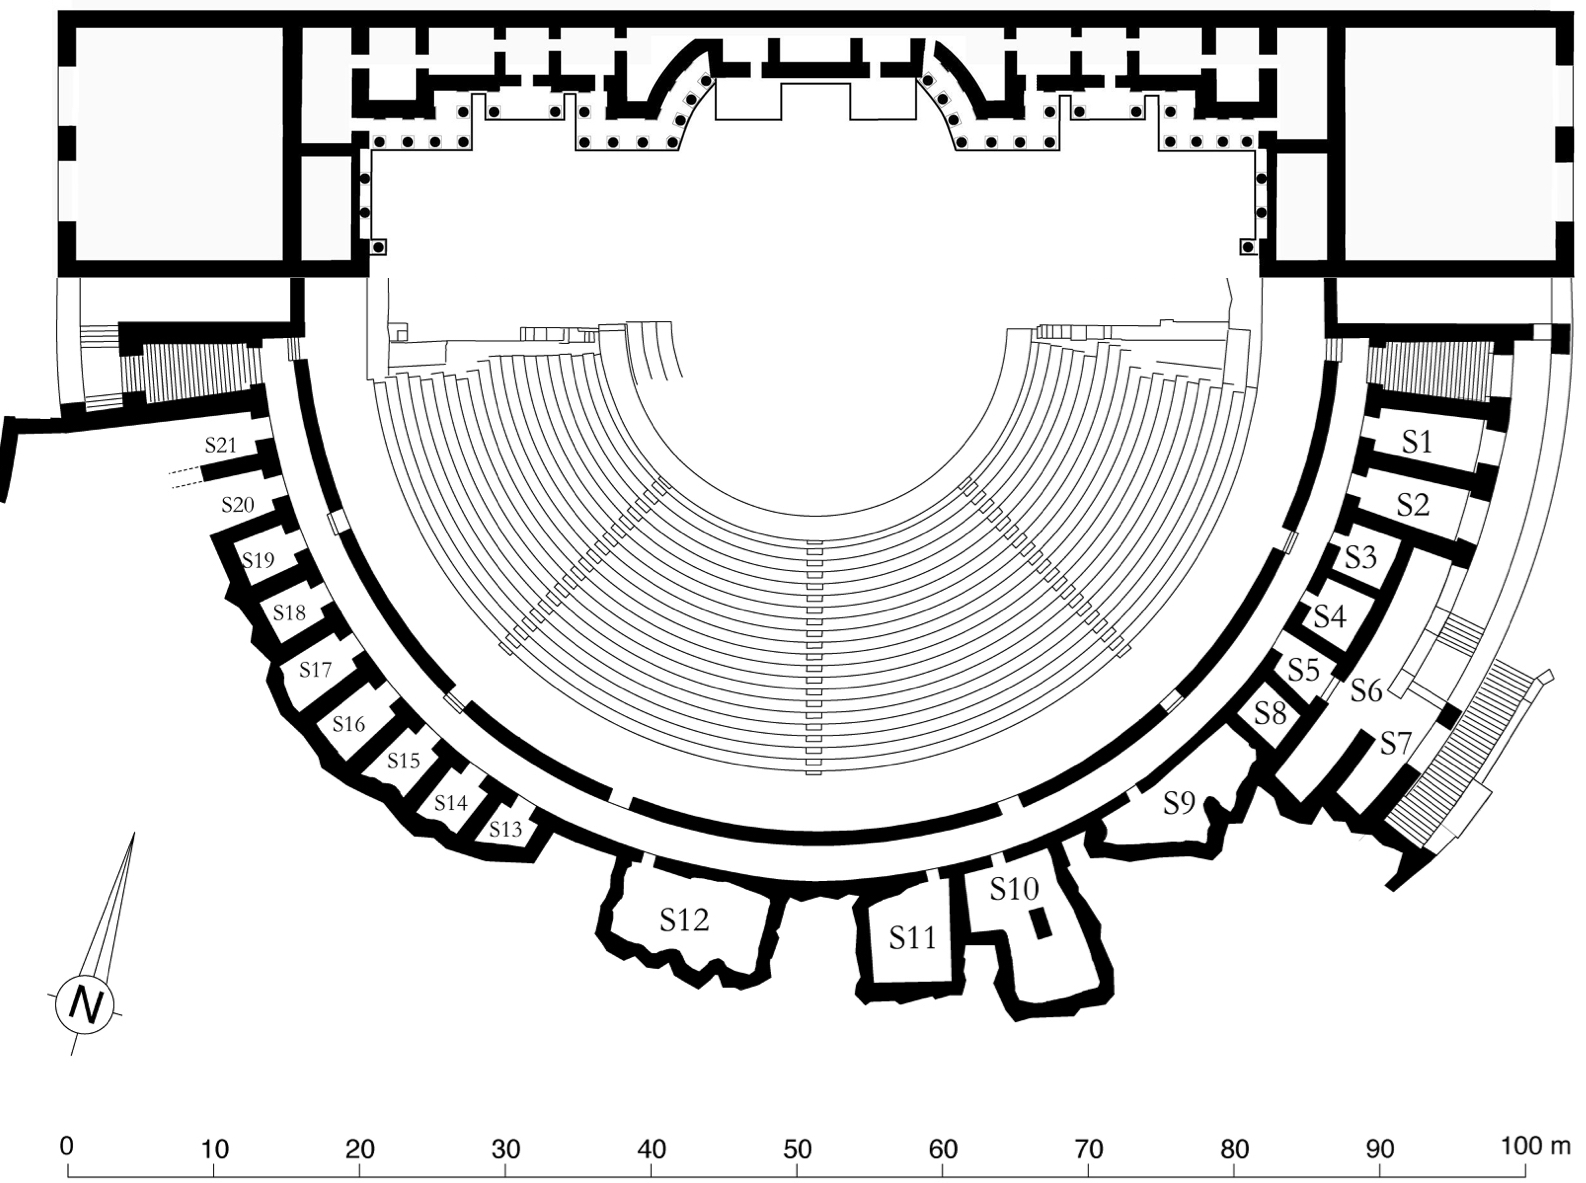
\includegraphics[width=\linewidth]{images/1erniveau}
		\caption[Vue de dessus - 1er niveau]{Plan du théâtre au niveau du premier ambulacre \cite[Pl. XVII]{orangePl}}
		\label{1erniveau}
	\end{figureth}		
		
Le deuxième \gls{maenianum}, ou \textit{media cavea}, repose, dans sa partie inférieure, sur l'\gls{ambulacre} du premier niveau et, dans sa partie supérieure, sur de la terre ou du remblai que complète, à proximité des \gls{aditus}, deux niveaux de chambres voûtées. Il comporte actuellement neuf gradins divisés en huit \gls{cuneus} par neuf escaliers ce qui semble être un choix acceptable au vu du corpus comparatif. Par ailleurs Caristie a relevé l'existence de cinq caissons de soutènement (C7 à C11 - fig. \ref{2emeniveau}) situés sous la \textit{summa cavea} et délimitant les passages permettant de se rendre au second \gls{ambulacre}. Celui-ci est souterrain dans la zone où la \gls{cavea} est adossée à la colline et construit sur deux niveaux de chambres voûtées dans sa partie la plus orientale. Il est directement accessible de l'extérieur par une porte à l'est et une autre à l'ouest.
		
	\begin{figureth}
		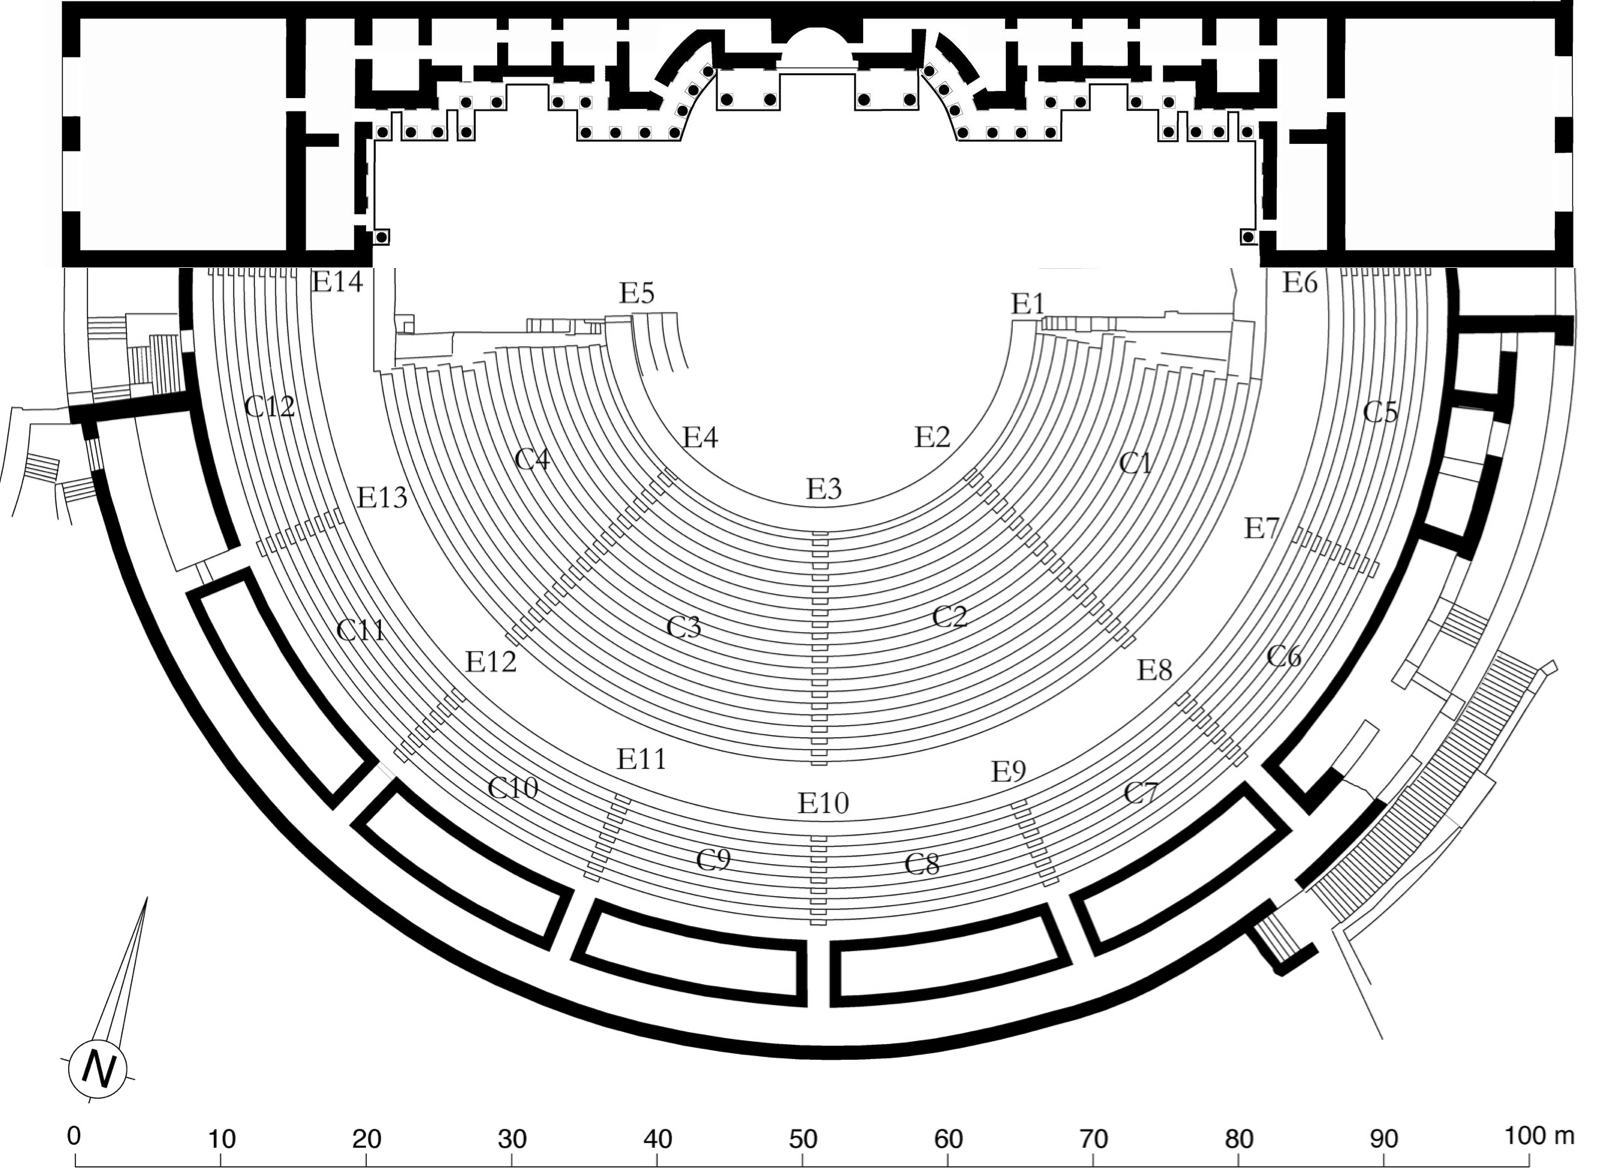
\includegraphics[width=\linewidth]{images/2emeniveau}
		\caption[Vue de dessus - 2ème niveau]{Plan du théâtre au niveau du second \gls{ambulacre} \cite[Pl. XVIII]{orangePl}}
		\label{2emeniveau}
	\end{figureth}		
		
		
Le troisième \gls{maenianum}, ou \textit{summa cavea}, comporte cinq gradins divisés également par neuf escaliers. On constate que la largeur de ses gradins diminue lorsqu'on s'élève, ainsi, ils ne mesurent plus que 72cm en moyenne sur le troisième \gls{maenianum}. Il était jadis couronné par une \gls{porticus isc}, dont l'existence est assurée par des traces sur les faces méridionales des murs des \glspl{basilique}. D'une largeur de 3m55 il semble qu'il n'ai été accessible que par les machiniste du \gls{velum} \cite{formige}. On trouve aujourd'hui des gradins sur échaffaudage à cet emplacement de même que sur les deux premières \glspl{precinction}. Une rue périphérique enclave la \gls{porticus isc} séparée par un mur que J-C Formigé avait percé de quatre portes au niveau des escaliers E9 à E12 (fig. \ref{2emeniveau} et \ref{3emeniveau}). L'accès en face de E9 est probable, non seulement parce qu'H. Daumet a noté une interruption du mur périphérique à cet endroit, mais aussi parce que le mur bordant la rue en amont est également percé d'une porte dans la prolongation de E9.


	\begin{figureth}
		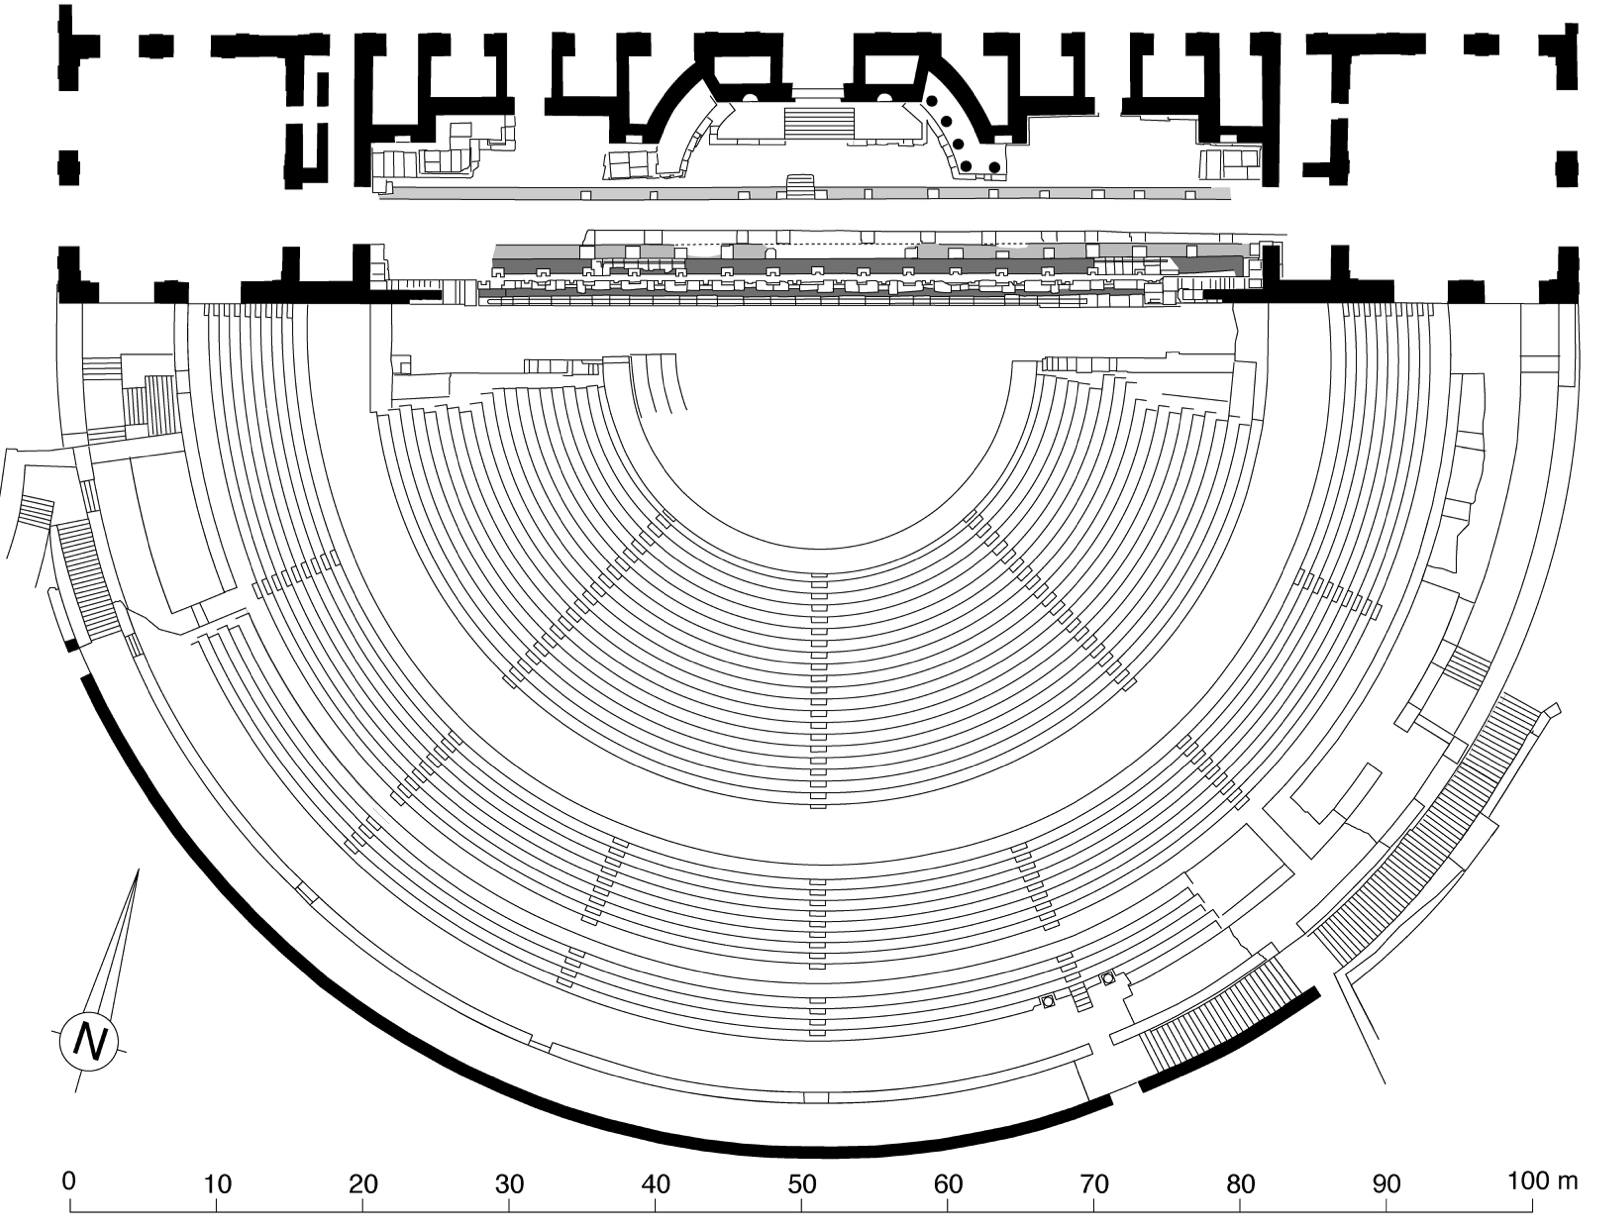
\includegraphics[width=\linewidth]{images/3emeniveau}
		\caption[Vue de dessus - 3ème niveau]{Plan du théâtre au niveau de la rue périphérique \cite[Pl. XIX]{orangePl}}
		\label{3emeniveau}
	\end{figureth}	
		
		
		\section{Les couvertures et le velum}
		
		\subsection{La couverture des \glspl{basilique} et du \gls{parascaenium}}
		
		La toiture qui figure aujourd'hui au-dessus des \glspl{basilique} et du \gls{parascaenium} (installée en 2006) reflète au peu près la proposition de restitution qu'avait fait A. Caristie à savoir un toit à double pente avec \gls{aretier} sur la diagonale partant de l'angle du mur arrière. L'étude de l'\gls{iraa} tend à corriger cette hypothèse en supposant plutôt la présence de deux toitures successives et, au-dessus de la cage d’escalier d’un petit toit à double-pente permettant non pas l’accès aux combles mais de monter sur le toit lui-même \ref{couvertureBadie}. Cette dernière hypothèse provient des traces symétriques situées au-dessus de la cage d’escalier orientale et donne de nouvelles pistes aux archéologues sur la façon de fonctionner des architectes de l'antiquité et les moyens d'entretiens du bâtiment dont ils disposaient. 
		Au niveau de la paroi sud de la \gls{basilique} la toiture fait une pente de 21° sur 14.22m et à partir du mur faisant jonction avec la cage d'escalier descend sur 15.44m jusqu'au niveau des bouches d'évacuation d'eau. 
		
		\begin{figureth}
			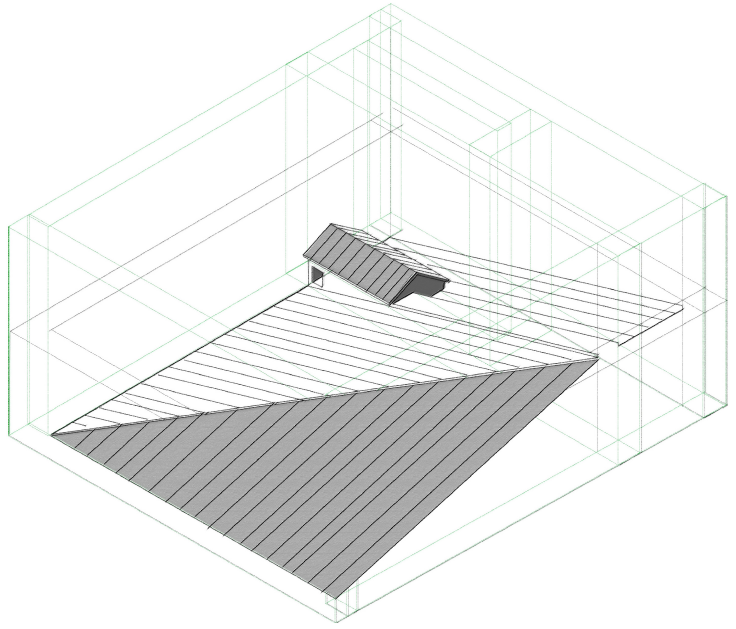
\includegraphics[width=\linewidth]{images/couvertureBadie}
			\caption[Toitures de basiliques par A.Badie]{Proposition de restitution des toitures de la \gls{basilique} occidentale, de la cage d'escalier et du \gls{parascaenium} \cite[Pl. XLVII]{orangePl}}
			\label{couvertureBadie}
		\end{figureth}	

		
		\subsection{La couverture du \gls{postscaenium} et du \gls{pulpitum}}
		
		Comme pour les toitures des \glspl{basilique} évoquées précédemment, le \gls{postscaenium} et le \gls{pulpitum} possèdent une couverture récente cette fois faite en métal. Le choix de cette toiture reste sujet à controverse car bien que l'acier présente de nombreux avantages face au bois (poids, résistance au temps, etc), il dénature l'aspect esthétique du bâtiment de part son anachronisme. La version antique n'a laissé aucun vertige en elle-même car elle devait être faite en matériaux périssable et semble avoir subit un ou plusieurs incendies. Néanmoins les études de A. Caristie puis de l'\gls{iraa} par la suite permettent d'entrevoir la forme de cette couverture. Premièrement, on distingue dans la partie sommitale du mur de scène des cavités d'encastrement permettant d'accueillir la charpente de la toiture elles-même couronnées par une série de déversoirs par lesquels s’échappait l’eau de pluie. Deuxièmement, on peut observer une saignée sur le mur occidental indiquant la pente de la partie supérieure de la charpente (fig. \ref{toitBadie}). Troisièmement on constate que le mur sud du \gls{postscaenium} (le front de scène) se terminait avec une pente de 19° d'après les marques laissées par un incendie sur les murs latéraux et ceci qui nous reflète la pente inférieure de la toiture. A. Carsitie a proposé une restitution de la couverture (fig. \ref{toitCaristie}) en s'inspirant des grues en bois utilisées à son époque et précise qu'il s'agit de "la combinaison qui" lui "a paru la plus vraisemblable, sous le rapport de la construction, pour la couverture du proscenium sans prétendre cependant que
ce soit la seule solution possible de cette intéressante question". Effectivement le rapport \cite{orangeTxt} conteste la forme triangulaire proposée par A. Caristie en faveur d'une forme parallélépipédique qui semble plus vraisemblable compte tenue du parallélisme des traces évoquées plus haut (fig. \ref{toitBadie}). Par ailleurs cela coïncide avec la présence d'ouvertures au sommet des murs latéraux permettant probablement d'atteindre la partie antérieur du comble alors que la proposition de A. Caristie les obstruait partiellement. Cette forme de toiture semble d'autant plus plausible au niveau architecturale qu'il en a été retrouvé des similaires dans les archives d'autres monuments. Cependant, il a été constaté que les cavités d'encastrement ont été plusieurs fois ajustées, agrandies ou rétrécie ce qui suppose qu'il y aurait eu plusieurs toitures installées au cours de la vie du bâtiment. Notre étude pour ainsi permettre de restituer différentes versions et de les comparer entre elles.
		
		
		\begin{figureth}
			\begin{subfigureth}{0.49\textwidth}
				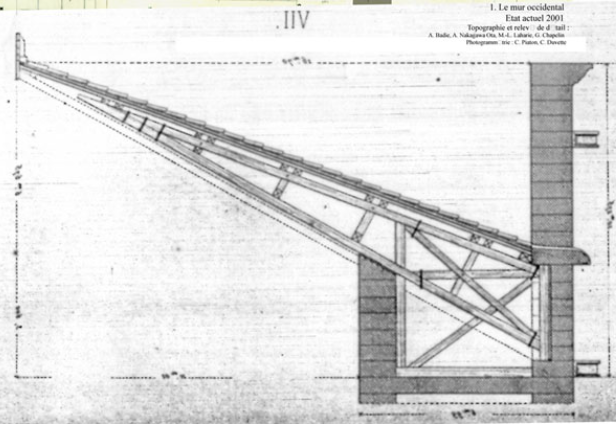
\includegraphics[width=\linewidth]{images/toitCaristie}
				\caption[Couverture de scène proposée par A.Caristie]{Proposition de restitution de la couverture de la scène par A.Caristie}
				\label{toitCaristie}
			\end{subfigureth}	
			\begin{subfigureth}{0.49\textwidth}
				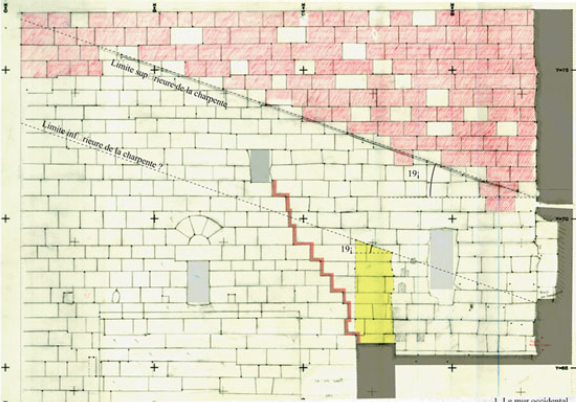
\includegraphics[width=\linewidth]{images/toitBadie}
				\caption[Relevé de la partie sommitale du retour ouest du front de scène]{Relevé de la partie sommitale du retour ouest du front de scène \cite[Fig. 24]{orangeTxt}}
				\label{toitBadie}
			\end{subfigureth}
		\end{figureth}
		
		
		\subsection{La couverture de la \gls{cavea}}
		
		Il est reconnu que les théâtres romains possédaient généralement un appareillage permettant de déplier au dessus des spectateurs de longues toiles appelées des \textit{vela} et communément assimilé à un ensemble unique : le \gls{velum}. Celui-ci permettait aux spectateurs d'être protégé du soleil et se déployait probablement partiellement en suivant le déplacement de l'astre notamment pour garantir une bonne ventilation. Nous savons d'après \cite{pline} que "ce fut seulement après Cléopâtre qu'on fit usage des toiles de lin pour donner de l'ombre dans les théâtres" \cite{formige}. Nous avons déjà évoqué plus haut les \glspl{console} permettant d'accueillir les mâts auxquels étaient accrochés les cordages. Il y en a douze au niveau du mur de scène et vraisemblablement tout autour du mur périphérique de la \gls{cavea} (dont il ne reste malheureusement aucune trace). Les modèles les plus courant représentent le \gls{velum} par un anneaux situé au dessus de l'\gls{orchestra} auquel sont attachés les cordages qui permette de le hisser par un système de poulie. Nous avons vu que les machinistes se plaçaient probablement au niveau de la \gls{porticus isc} pour dans un temps hisser l'anneau puis ensuite déployer certaines \textit{vela} au moment approprié.  
		
		Le théâtre d'Arles présente un certain nombre de trous au niveau de son premier gradin qui semblent avoir accueilli des mâts de soutient pour le \gls{velum}. \`{A} coté de ceux-ci on trouve de plus petits trous probablement utilisés pour fixer les cordes. Cette particularité a peu été observer par ailleurs et pourrait être du à la présence d'un fort mistral dans cette région et donc pourrait également avoir été mis en place à Orange.
		A. Caristie propose une restitution de \gls{velum} avec un anneau semi-circulaire et 67 mâts autour de la \gls{cavea} (fig. \ref{velumCaristie}).
		
\begin{figureth}
		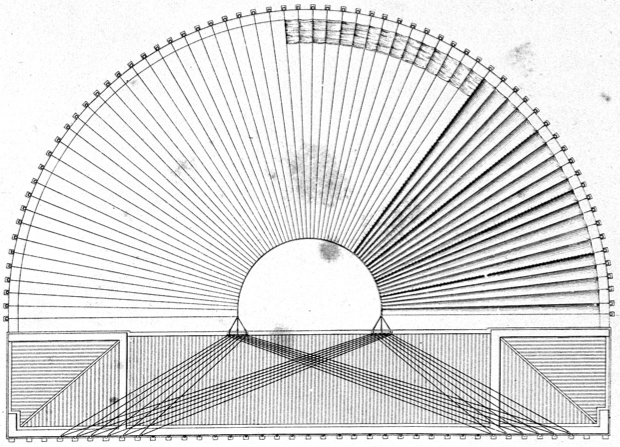
\includegraphics[width=\linewidth]{images/velumCaristie}
		\caption[Velum]{Proposition de restitution du velum d'Orange par A.Caristie}
		\label{velumCaristie}
\end{figureth}		















	\chapter{Modélisation}
		\citationChap{
			Les détails font la perfection et la perfection n'est pas un détail
		}{Léonard de Vinci}
		\minitoc
		\newpage
		
		\section{Introduction}
		Pour pouvoir étudier un monument dans ces moindres détails de nombreux chercheurs s'orientent aujourd'hui vers la modélisation 3D. Effectivement, jusqu'à ces quelques dernières années, les analyses architecturales antiques étaient principalement menées à l'aide de plans, de dessins, ou bien de maquette à échelle réduite. Mais les outils numériques disponibles aujourd'hui comportent de nombreux avantages par rapport à ces anciennes techniques. Tout d'abord, il est possible d'obtenir les mêmes informations qu'avec des dessins ou des maquettes en terme de côtes, formes, aspect. Mais se rajoute à cela qu'à partir d'un modèle numérique unique, on peut sélectionner les quelles informations l'on souhaite étudier tout simplement en changeant l'objet affiché, la vue ou le mode d'affichage. On peut par exemple observer un monument par vu du dessus avec ses cotes en étudier ainsi le plan 2D correspondant. Mais on peut également réaliser une impression 3D de l'objet pour en avoir une maquette physique à l'échelle réduite. Un seul et même outil permet donc d'obtenir l'ensemble des informations que l'on souhaitait acquérir par le passé tout en améliorant leur qualité grâce à la précision des ordinateurs. Un modèle numérique 3D peut par ailleurs être utilisé par des logiciels de calcul ou de simulation afin de tester des comportements physiques tels que les écoulement de fluide ou l'acoustique par exemple. Il en est de même pour les questions architecturales d'agencement de décor ou de portance par exemple. Il permet également de réaliser des animations (déplacement de personnages, ouverture de haut-vents, ...) ou des visites immersives grâce aux technologies de réalité virtuelle. On peut alors visualiser son objet d'étude dans son ensemble ou bien partie par partie à l'aide de technologies telles que les écrans 3D, les caves (écrans géants parabolique ou cubiques) ou les casques de réalité virtuelle nous plongeant littéralement au coeur de l'objet.

Il existe bien entendu de nombreuses limites à la numérisation 3D car cette technique est relativement récente et beaucoup de développement sont en cours. La principale contrainte est la puissance de calcul des ordinateurs et leur espace de stockage qui doivent prendre en charge de très grandes quantités de données.

Pour virtualiser des monuments, il existe principalement deux techniques le plus souvent utilisées. La première consiste à réaliser un nuage de point à l'aide d'appareils de mesure (laser, appareils photo, ...) à la manière d'un scanner. Prenons l'exemple de la photogrammetrie qui est aujourd'hui largement répandue dans la restitution numérique de monument. Il s'agit de photographier l'ensemble du bâtiment sous tous ses angles en s'assurant que chaque photo a une partie commune avec une autre. Les logiciels de traitement peuvent alors corréler les photos les unes avec les autres et recréer l'image en trois dimensions. Cependant, la limite de cette technique est que plus la précision est grande, plus le volume de donnée à traiter est conséquent et rend les calculs difficiles. C'est pourquoi nous avons utiliser la deuxième méthode dite de \gls{cao}. Il s'agit de retranscrire le monument par des formes géométriques 3D plus ou moins complexes.

Il existe cependant un certain nombre de logiciels permettant d'utiliser cette technique et nous citerons parmi les plus connus : \textit{AutoCAD, CATIA, SketchUp, 3DSMax}. Après une étude comparative, le choix s'est porté sur le logiciel \textit{Blender} car celui-ci possède l'avantages d'être :

\begin{itemize}
	\item gratuit
	\item multiplatforme (Windows, Mac, Linux)
	\item modulaire (de nombreuses fonctionnalités peuvent y être ajoutée selon les besoins)
	\item suivit et commenté par une large communauté
\end{itemize}

Par ailleurs, Blender : 
\begin{itemize}
	\item permet un rendu réaliste, voir photo-réaliste) notamment grâce au texturage
	\item permet de réaliser des animations et des vidéos
	\item utilise des effets physiques tel que la gravité, la déformation de type tissu, l'écoulement de fluides ...
	\item peut exporter les maillages sous différents formats couramment utilisés (obj, fbx, stl, ...)
	\item permet le développement de script en python
\end{itemize}

Toutes ces spécificités vont être utilisées dans le projet et c'est pourquoi c'est ce logiciel qui a été choisi. Il comporte néanmoins quelques limites notamment sa difficulté de prise en main, le fait qu'il soit peu utilisé dans le milieu architectural et que son "\textit{game engine}" soit de moins bonne qualité que certains de ses concurrents (Unity ou Unreal Engine par exemple). En ce qui concerne ce dernier point, cela n'est pas gênant car Blender peut exporter des modèles texturés dans Unity ou Unreal pour des visites virtuelles de très haute qualité.

Dans ce chapitre nous allons donc présenter comment le théâtre antique d'Orange a été modélisé avec Blender, quelles ont été les difficultés soulevés et les astuces utilisées. Il sera préciser quels sont les informations architecturales et archéologiques que concaténe le modèle numérique ainsi que les sources qui ont permis de les implémenter.
Avant de détailler uns par uns les éléments modélisés, il faut voir le modèle dans son ensemble et notamment dans son repère. Sur le plan XY, c'est à dire le plan de l'horizon on choisi le point (0,0) au centre du demi-cercle formé par l'\gls{orchestra}. Nous faisons ce choix car cette dernière ainsi que l'ensemble de la \gls{cavea} possède un centre de révolution et il sera plus pratique par la suite, notamment au moment d'appliquer des outils automatiques de placer celui-ci au centre du repère de Blender. Concernant Z ou d'élévation, nous utiliserons les relevés d'altitude présents dans le rapport \cite{orangePl} et donnant des élévations géoréférencées par rapport au niveau de la mer. Le plan de l'\gls{orchestra} par exemple se trouve donc à 40m sur l'axe des Z.


	\section{La cavea et ses substructures}  \label{La cavea et ses substructures}


La \gls{cavea} est le premier élément que nous modélisons car, comme stipulé plus haut, son centre de révolution est situé à l'origine du repère XY. La modélisation se fait à partir de la figure \ref{coupeCavea}. La première chose à noter est que sur ce plan, on ne connait pas la distance par rapport au centre de révolution. Par contre on sait que la paroi extérieure est au même niveau que la bordure des \gls{basilique}, c'est à dire à 51,96m du centre de part et d'autre (en prenant la moitié de la longueur totale du mur de scène). On part donc de cette paroi extérieure pour dessiner sur blender la coupe de la \gls{cavea} en suivant les cotes indiquées. Cependant plusieurs points posent difficulté. Premièrement les gradins sont représentés de manière hypothétique. Pour connaitre leur largeur dans le plan, on doit utiliser les quatre lignes de cotes horizontales. Or pour les deux lignes arrivant du niveau du mur du podium au dessus du deuxième \gls{maenianum} on a deux informations contradictoires. D'une part, nous avons 8m91 (125+260+113+290+103) et d'autre part 8m69 (35+92+259+483) soit 22cm de différence. Or on estime qu'il n'est pas crédible que le mur soit incliné de la sorte. Trois causes d'erreur sont possibles. Premièrement la mesure qui a été faite a été mal reportée et le document présente une coquille. Deuxièmement, les mesures ne sont pas toutes effectuées sur un même plan de coupe et d'un endroit à l'autre de la cavea, l'épaisseur des murs peut effectivement varier. Troisièmement, la mesure est exacte mais les pierres s'étant érodées par endroit, on observe des fluctuations d'épaisseur des murs qui n'avait pas lieu à l'origine du théâtre. Pour trancher sur la décision nous adoptons la règle suivante :

\begin{theo}\label{epaisseur}
	Lorsque deux cotes sont contradictoires on utilise celle correspondant à la plus grande épaisseur de pierre.
\end{theo}

Cela permet donc de trancher dans le choix des cotes tout en prenant en compte la possibilité que les pierres se soient érodées.

\begin{figure}[!h]
	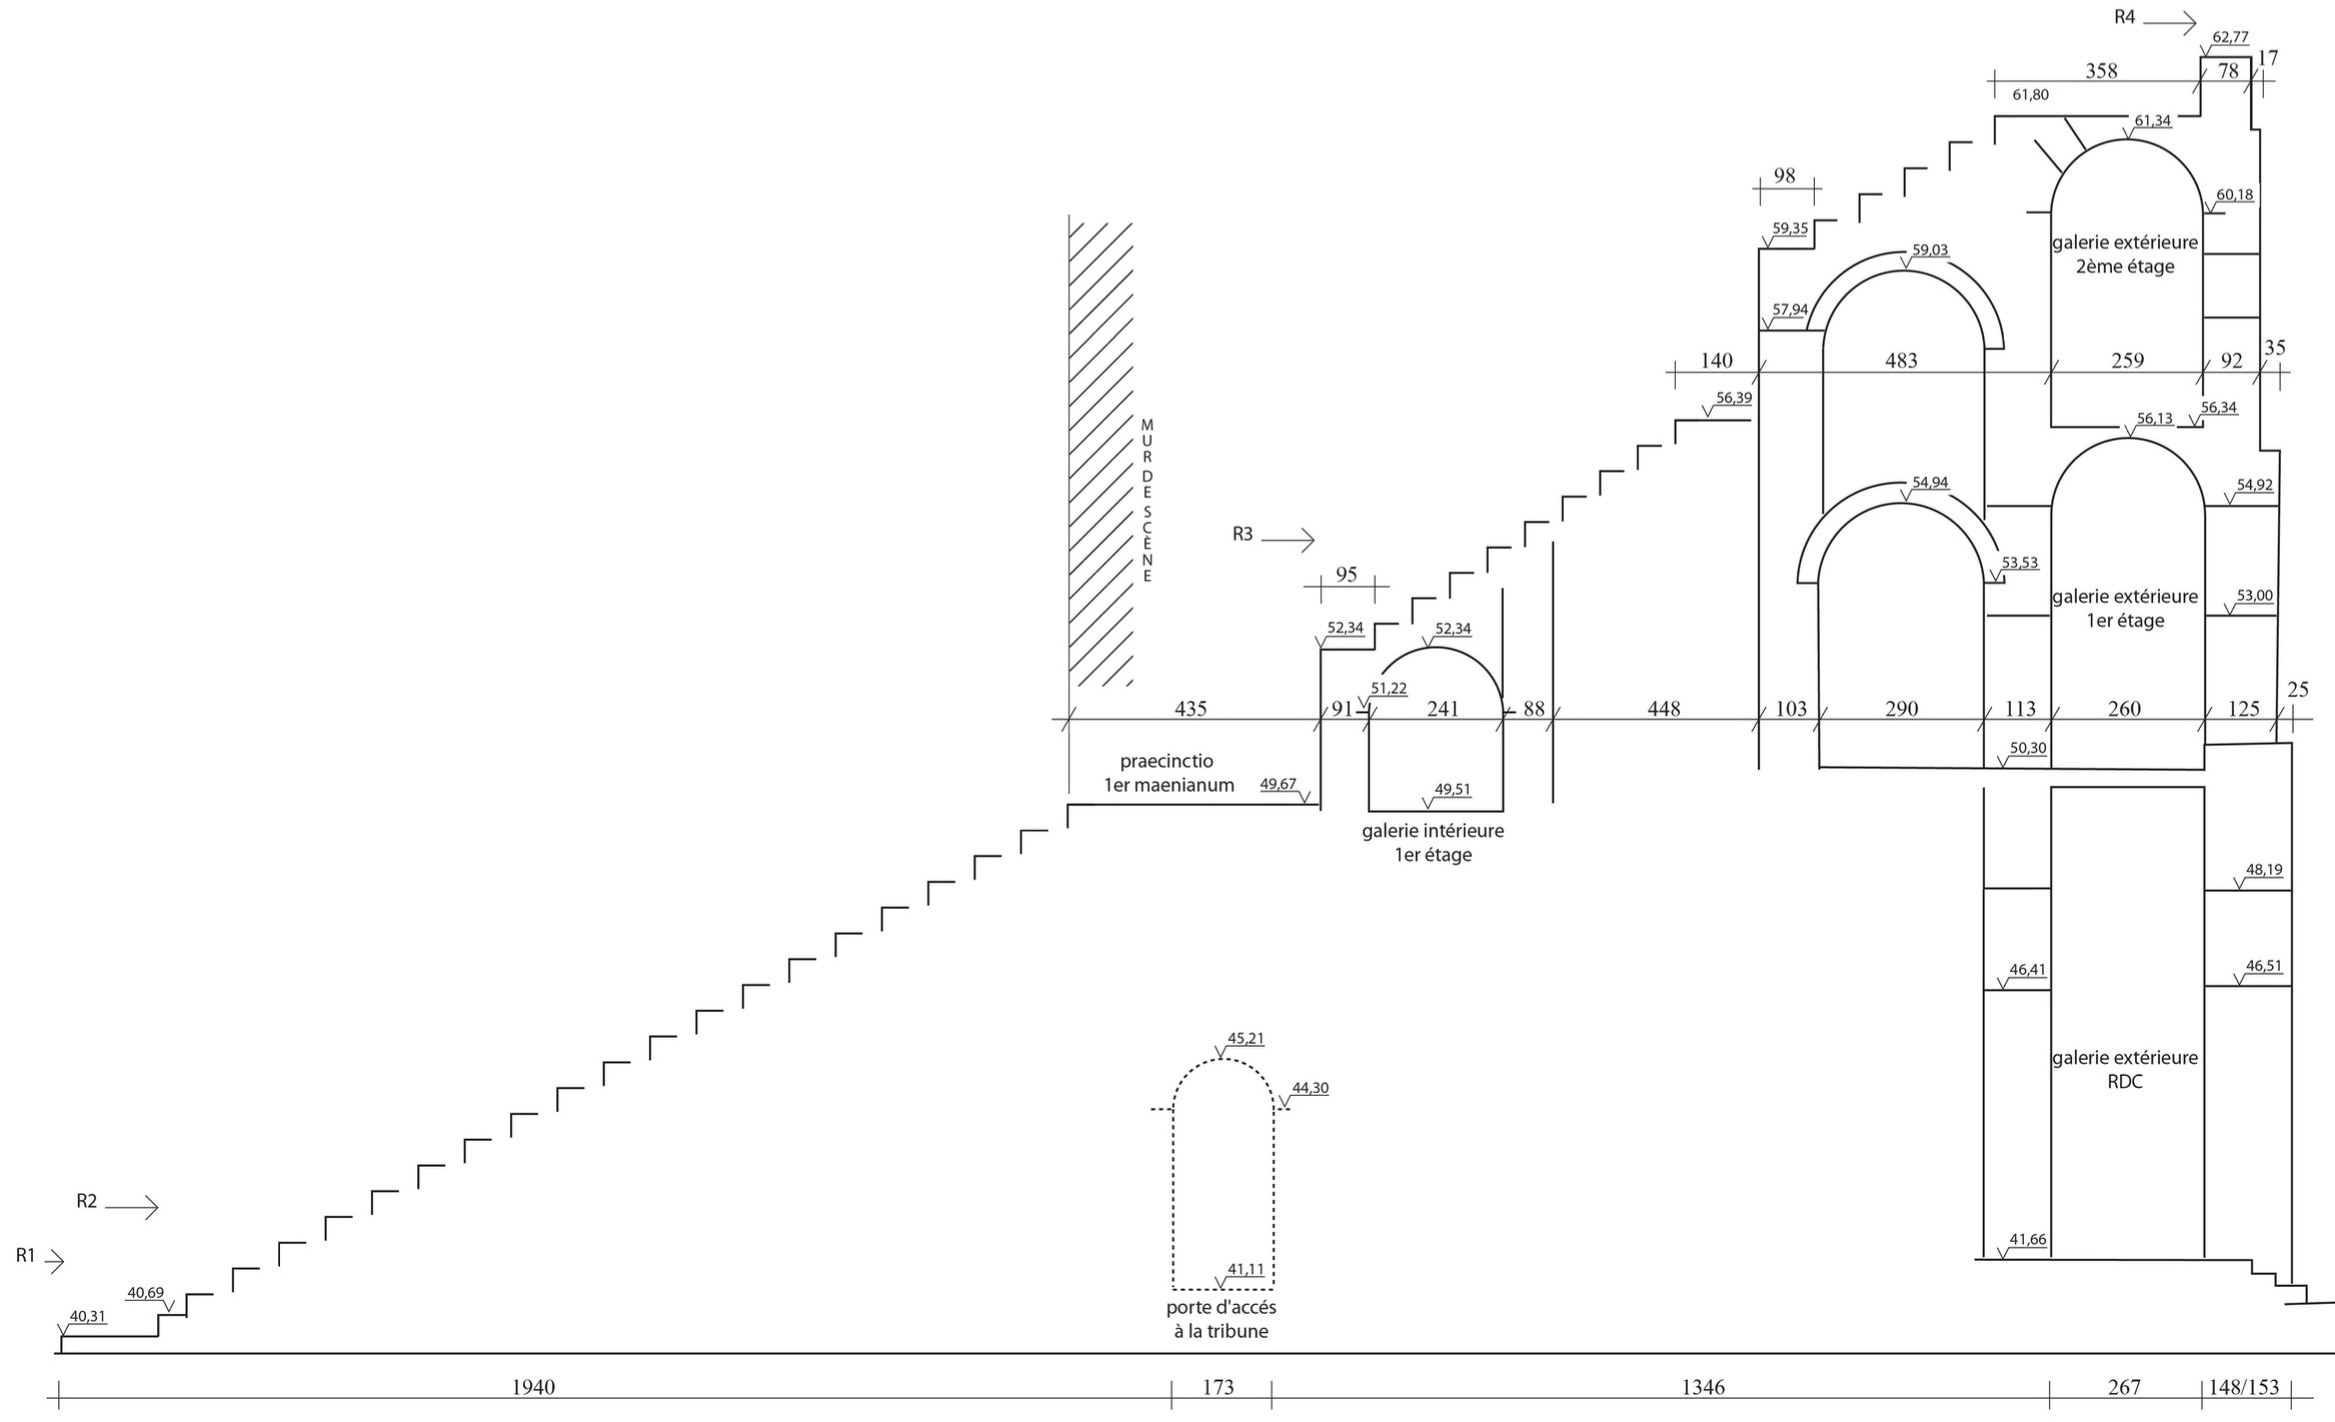
\includegraphics[width=\linewidth]{images/CoupeCavea}
	\caption[Coupe théorique sur la \gls{cavea}]{Coupe théorique sur la \gls{cavea} \cite[Pl. LX]{orangePl}} 
	\label{coupeCavea} 
\end{figure} 

Pour cette même longueur, A.Carisite donne des mesures encore différentes (455+270+95). En ajoutant le décrochage de 35cm on obtient 8m55. On voit donc bien que la cavea ne pourra pas être modélisée avec une précision supérieure à quelques dizaines de centimètres on utilisant des cotes communes sur toute la circonférence. Pour obtenir un résultat plus réaliste il faudrait effectuer de nouvelles campagnes de mesure en un nombre significatif de points. Néanmoins, les restaurations de la cavea ayant été très conséquentes, il semble extrêmement difficile de remonter à la structure initiale avec grande précision.

Pour créer la substructure du troisième maenianum nous appliquons donc la règle \ref{epaisseur} explicitée plus haut et nous nous référerons à ce plan théorique pour connaitre les élévations. Lorsque celles-ci ne sont pas chiffrées et qu'on ne les retrouve pas dans un autre document, nous obtenons la valeur par mise à l'échelle du plan. Nous modélisons également les trois niveaux de galeries qui seront solidaires de cet objet. Les caissons de soutènement situés sous le troisième \gls{maenianum} sont par contre modélisés séparément. Effectivement, contrairement à la cavea, on ne va pas les extruder à 180° mais chaque caisson va être séparé de son voisin laissant l'espace pour les vomitoires du deuxième ambulacre. Effectivement, A. Caristie restitue dans ses plans six de ces caissons de soutènement (dont un incomplet) validant leur origine antique. Ainsi on utilise, à partir de la figure \ref{CoupeCavea} les cotes en deux dimensions de ses caissons qu'on répète huit fois avec un angle de 21,95° et que l'on extrude à l'aide d'un \gls{screw} sur 19,2°. On fait ensuite subir une rotation globale à l'ensemble des huit caissons afin qu'ils soient symétriques par rapport à l'escalier central de la cavea (quatre de chaque coté). 

Pour réaliser substructure du deuxième maenianum on complète le modèle afin que la première precinction arrive à l'affleurement du mur de scène. Là encore on trouve un problème de cotes puisque la largeur de la basilique est, d'après la figure \ref{cotes}, de 1,34+14,22+1,17+3,55+1,19 soit 21,47m. Or si on calcule 4,35+0,91+2,41+0,88+4,48 on obtient 13,03m. En les ajoutant aux 8,91m déjà modélisés, on arrive à 21,94m soit 47cm de différence. A. Caristie donne 8m entre les podium du deuxième et du troisième niveau contre 8m68 pour M. Fincker et J.M Labarthe. Les deux plans sont par contre cohérent à 5cm près concernant la largeur de l'ambulacre ainsi que l'épaisseur de ses murs. C'est donc au niveau du ramblais soutenant la partie supérieur du deuxième maenianum que se trouvent les écarts de mesure. On part donc de l'angle de la basilique pour créer la precinction le podium et l'ambulacre du premier niveau. La precinction du deuxième niveau est par contre créée à partir du podium du deuxième niveau car on connait sa longueur et son élévation. 

Il reste la substructure du premier maenianum. Ici encore la longueur des gradins n'est pas stipulée. Par contre, A.Caristie nous dit que le repose-pied se trouve à 14m95 du centre de la cavea et que le podium du premier niveau se trouve 20m plus loin. On constate qu'en enlevant les 4m35 de la première precinction aux 34m94 de Caristie on obtient 30m59 ce qui est proche des 30m49 de demi-longueur du mur de scène auquel on ôte la basilique (51m96 - 21m47). En considérant que les gradins ont tous la même largeur pour au sein de chaque maenianum, il ne manque que l'information de la largeur du marche pied et de la couverture du caniveau pour terminer cette partie. Ces dimensions sont encore une fois obtenues par mise à l'échelle des plans.

%\begin{figure}[!h]
%	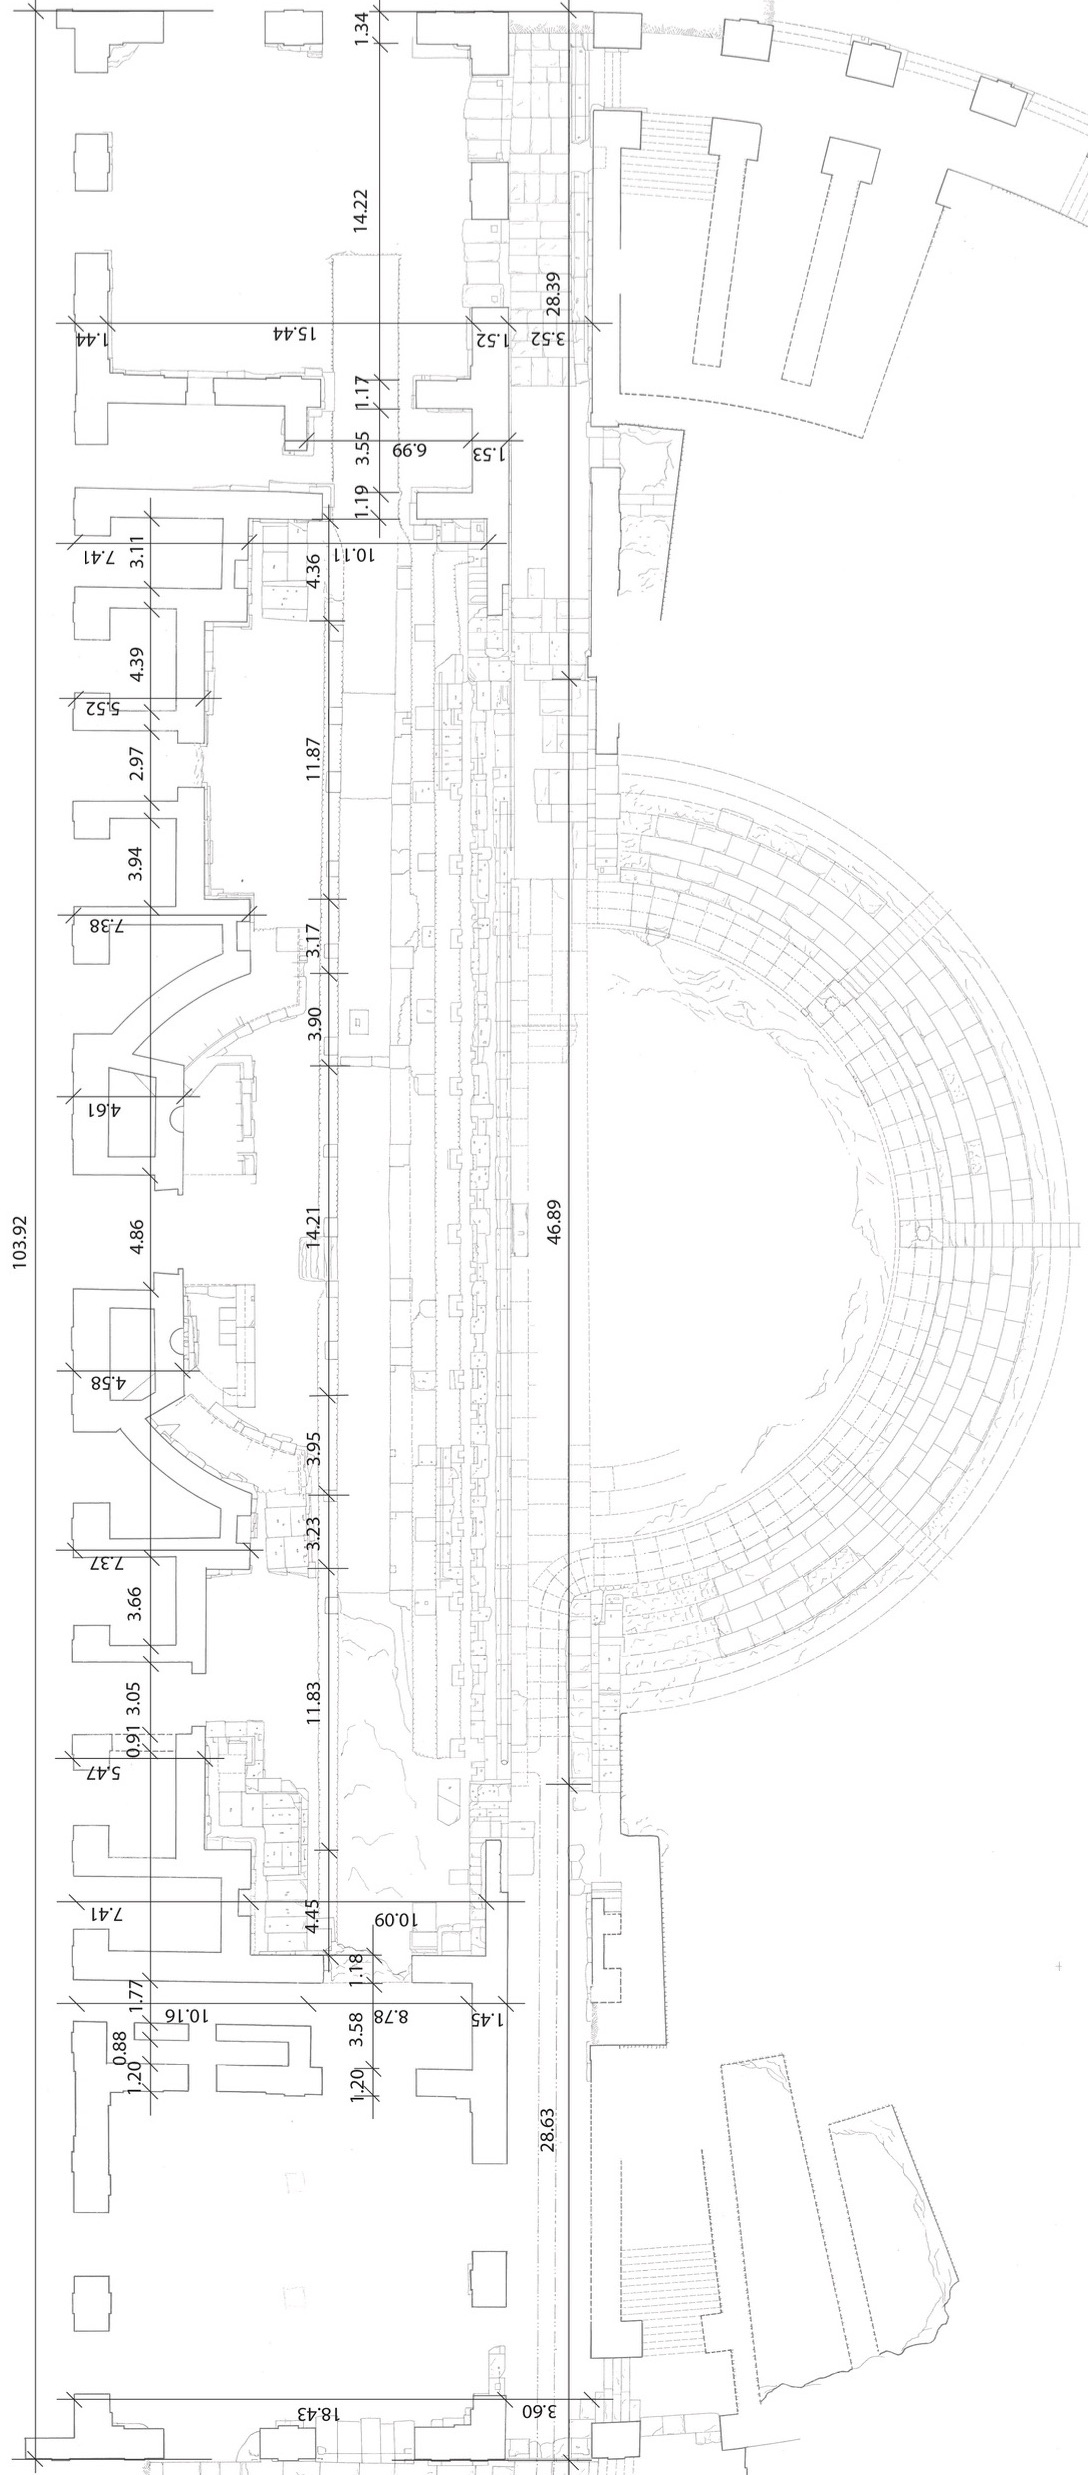
\includegraphics[height=0.8\paperheight]{images/cotes}
%	\caption[Plan du rez-de-chaussée au bâtiment de scène]{Plan du rez-de-chaussée au bâtiment de scène \cite[Pl. XXI]{orangePl}}
%	\label{cotes} 
%\end{figure} 
		
Une fois ce plan de coupe réalisé on utilise le \gls{screw} pour l'obtenir en volume sur un hemicicle. On peut alors modéliser les arcades donnant sur l'extérieur. Celles-ci sont créées en élévation grâce à cette planche également. Leur largeur de 3,419m est donnée par le plan de A.Caristie \cite[Pl. XXXIII]{orangePl} en estimant qu'elles ont une largeur identique aux entrées des \gls{aditus}. On peut considérer que les arcades des trois niveaux ont une hauteur différente mais une largeur constante car les parois internes des \gls{aditus} ne présentent pas de marque contredisant cette hypothèse. Si les arcades avaient fait tout le tour de la cavea c'est à dire 180° dans le cas où il le théâtre n'aurait pas été adossé à la colline, il y aurait eu 31 arcades sur chaque niveau. Un triplet d'arcades verticales est donc répétées 31 à l'aide d'un \gls{array} avec un angle de 6,13°. Celles-ci sont ensuite soustraites à la \gls{cavea} par un \gls{boolean}. Il est bon de noter que pour pouvoir utiliser le \gls{boolean} il faut au préalable appliquer le \gls{screw} (c'est à dire rendre permanent) puis de fermer le maillage. Au niveau de la première et deuxième \gls{precinction} on perce la structure à l'aide d'un \gls{boolean} pour créer les \gls{vomitorium} qui permettent d'accéder aux ambulacres. La forme qui va être soustraite à la cavea se compose d'un pavé droit créant un trou rectangulaire au niveau du podium puis d'un demi-cylindre extrudé permettant de créer un couloir vouté allant jusqu'à l'ambulacre. Ces passages sont disposés dans l'espace entre deux caissons. La forme est donc répétée avec un angle de 21,95° et la première forme un angle de 2° avec l'axe des x. On utilise donc le même objet de référence pour leur faire subir leur répétition de révolution grâce au \gls{array}. Le niveau bas est au niveau de la \gls{precinction} et le niveau haut arrive à 50cm en dessous du podium en considérant que l'espace au dessus du vomitoire est du même ordre de grandeur qu'un gradin. 

Une porte venant des aditus permet aux spectateurs de se rendre à mi hauteur de l'\textit{ima cavea}. Celle-ci mène à des escaliers qui n'ont pas été restaurés mais dont le plafond vouté est visible aujourd'hui (voir figure \ref{parodos}). Pour cet escalier, on sait que la première marche commence à 41,11m d'altitude et la dernière arrive à 45,58m. Or cet escalier débouchait probablement au dixième gradin, à la jonction où la partie basse de la cavea s'arrête et où la partie haute est soutenue pas l'aditus. On a donc 20 marches d'une hauteur de 22,35cm. \`{A} partir de la première marche, que l'on ajuste en longueur, et l'aide d'un \gls{array}, on complète l'escalier pour arriver au 10\up{e} gradin. On perce alors la cavea avec un objet représentant l'ouverture dans les gradins. A compléter ...


\begin{figure}[!h]
	\centering
	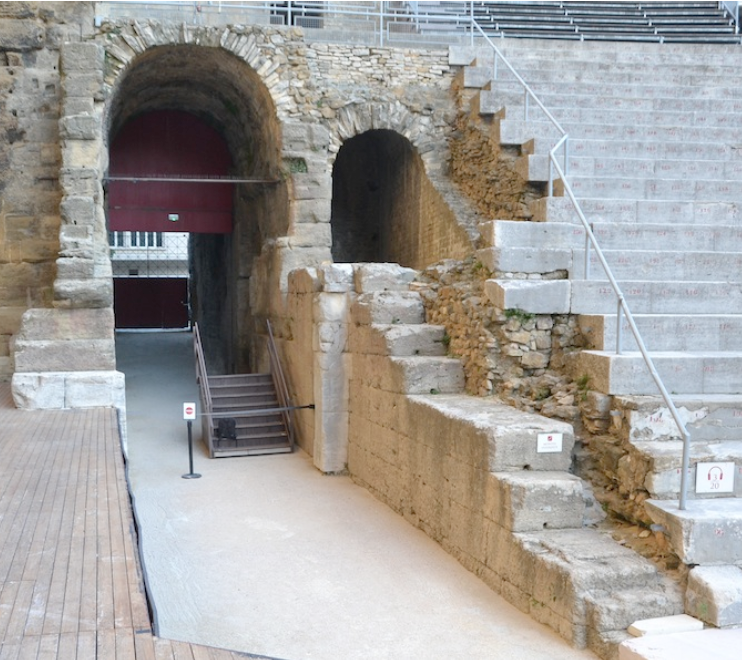
\includegraphics[width=0.5\textwidth]{images/parodos}
	\caption[\Gls{parodos} oriental et entrée menant àl'\textit{ima cavea}]{\Gls{parodos} oriental et entrée menant àl'\textit{ima cavea} \cite[fig. 418]{orangeTxt}} 
	\label{parodos} 
\end{figure}

\`{A} l'est et à l'ouest, le deuxième triplet d'arcades après l'\gls{aditus} donnait sur un escalier permettant d'accéder au premier \gls{ambulacre}. L'escalier oriental (fig. 435) a été restauré avec 31 marches par J.-C. Formigé, qui l'a fait aboutir dans l'ambulacre à un niveau de sol séparé par 4 marches de celui de la première précinction.  A. Caristie restituait un escalier de 24 marches conduisant à un premier ambulacre, dont le niveau de sol aurait été beaucoup plus bas que celui de la première précinction (pl. VI). Une dizaine de
marches aurait permis d'aller de l'ambulacre à la précinction.
Du côté ouest, J.-C. Formigé a restauré un escalier de 32 marches conduisant à
l'ambulacre (fig. 428)


		\section{Maenianum} 

Les maenianum, c'est à dire les gradins, sont modélisés séparément de la cavea. Chacun des trois maenianum est modélisé à partir d'un objet plan de forme quasi-triangle créé d'après la forme du morceau de gradin antique apparent dans le théâtre (figure \ref{coupeGradin}). Les gradins étaient à priori assemblés à partir de blocs rectangulaires sciés en deux sur une diagonale décalée d'une dizaine de centimètre à partir de l'angle. Ce méplat permet de poser les blocs les uns sur les autres. Le reste de leur longueur reposaient sur de l'\textit{opus caementicium}, sorte de remblai constitué de mortier et de tout-venant qui n'est pas modélisé. 

\begin{figure}[!h] 
	\begin{subfigureth}{0.49\textwidth}
		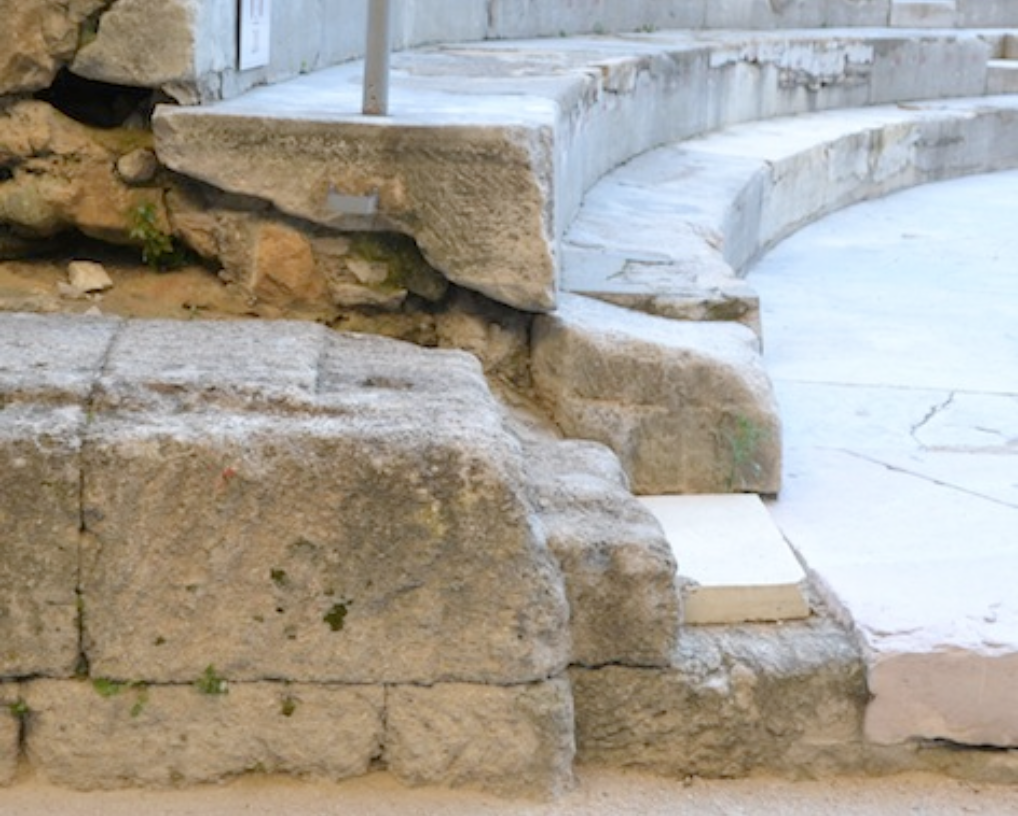
\includegraphics[scale=0.3]{images/gradinCoupe}
		\caption[Repose pied et premier gradin du premier \gls{cuneus}]{Le repose pied et le premier gradin du premier \gls{cuneus} : vu de l'extrémité nord avec au premier plan, le mur bordant l'\gls{aditus} est} 
		\label{coupeGradin} 		
	\end{subfigureth}	
	\begin{subfigureth}{0.49\textwidth}
		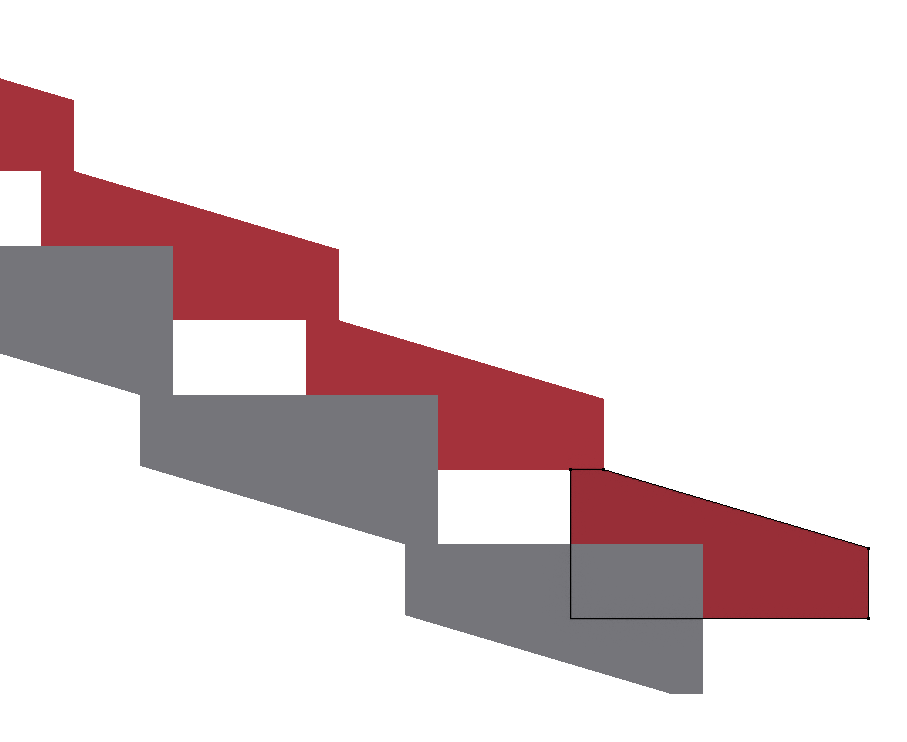
\includegraphics[scale=0.3]{images/escaliers}
		\caption[Modélisation des \gls{maenianum}]{Modélisation des \gls{maenianum} et de l'emprunte des escaliers à retirer après application des modifers Array et Screw}
		\label{modelMaenianum} 		
	\end{subfigureth}	
\end{figure}

\`{A} partir de ce plan, on applique un \gls{array} selon le nombre de gradins par maenianum, soit respectivement 19, 8 et 4 (la precinction faisant office de gradin supplémentaire). On adapte ensuite la longueur et la hauteur pour pouvoir encastrer le meanianum complet dans la cavea précédemment modélisée. Le premier gradin est placé à 15m35 du centre de la cavea laissant un repose pied de 40cm. On peut alors utiliser ensuite un \gls{screw} pour extruder la forme sur 180°. De la même façon on extrude les formes rectangulaires du repose pied situé devant le premier gradin ainsi que la couverture de caniveau. Au dessus de aditus on duplique la forme de base des trois maenianum pour en faire une partie linéaire de 3,6m à l'aide d'un \gls{solidify}. Les deuxième et troisième maenianum sont complets tandis que le premier ne comporte que les gradins 10 à 14. Ils sont symétrisés grace à un \gls{mirror}.

En ce qui concerne les escaliers, chaque marche mesure la moitié de la hauteur d'un gradin. Il s'agit alors de creuser chaque gradin sur son coin extérieur. Pour cela, pour chaque meanianum, on duplique le gradin de base, on lui fait effectuer une rotation de 180° autour de sa normale et on place son coin extérieur au centre du gradin (voir figure \ref{modelMaenianum}. On applique alors le même \gls{array} que pour les gradins pour répéter la forme sur la hauteur du maenianum. On utilise ensuite un \gls{solidify} pour donner à l'escalier sa largeur. Cette valeur est fixée d'après la \cite[Pl. XIX]{orangePl} mais reste modifiable. On utilise à nouveau un \gls{array} pour répéter de manière circulaire les escaliers autour du centre de la cavea. On a ainsi cinq escalier au niveau du premier maenianum et neuf au niveau des deuxième et troisième. L'escalier de référence est sur l'axe X (donc en y = 0). Pour le premier maenianum on le repéte tous les 45°. Pour les deuxième et troisième maenianum, l'escalier de base est repété comme les caissons et les vomitoires avec un angle de 21,95° en faisant faire une rotation au premier de 23,95° par rapport à l'axe X. Il y a néanmoins une subtilité pour ce qui concerne les marches alignées avec les \gls{parodos}. Pour le premier manenianum, ces marches ne sont pas centrée sur l'axe des x mais décalée de la moitié de leur largeur. Les dix premiers gradins s'arretant en y = 0 on aurait eu des marches deux fois trop étroite à cet endroit de même qu'au niveau de la tribune. Pour les modéliser, il suffit de dupliquer l'objet de base utilisé pour soustraire les marches et de lui appliquer son \gls{solidify} uniquement avec un offset de -1 permettant de l'élargir que d'un coté et non de part et d'autre. On effectue la même démarche pour le repose pied que pour le premier maenianum. Les les deuxièmes et troisième maenianum, les traces présentes sur le mur des basiliques indiques que les escalier étaient en bordure de gradin. Les marches alignées avec les \gls{parodos} sont donc creusées en utilisant une copie de la forme de base décalée de 3,6m sur l'axe Y. On utilise un \gls{mirror} pour les rendre symétrique par rapport au centre de la cavea.
Une fois les modifiers appliques sur les maenianum et le maillage fermé, on peut soustraire les marches d'escaliers à l'aide d'un \gls{boolean}. On soustrait également une marche sur chaque precinction de l'objet cavea. Le premier maenianum est egalement percé tout comme la cavea au niveau de l'entrée menant au dixième gradin.


		
		\section{Aditus} 
		
Les aditus sont en réalité une extension de la cavea qui se prolonge de manière rectiligne sur l'axe y (sud-nord à peu près). Il est important pour le model numérique qu'il y ai jonction entre l'objet "cavea" et les objet "aditus" en tout cas sur la partie commune c'est à dire partout excepté au niveau de la tribune et des \gls{parodos}. Or les relevés (voir figure \ref{aditusOccidental} et \ref{aditusOriental}) stipulent des mesures qui différents d'un aditus à l'autre et également par rapport à la cavea théorique (figure \ref{coupeCavea}).

		
\begin{figureth}
	\begin{subfigureth}{0.49\textwidth}
		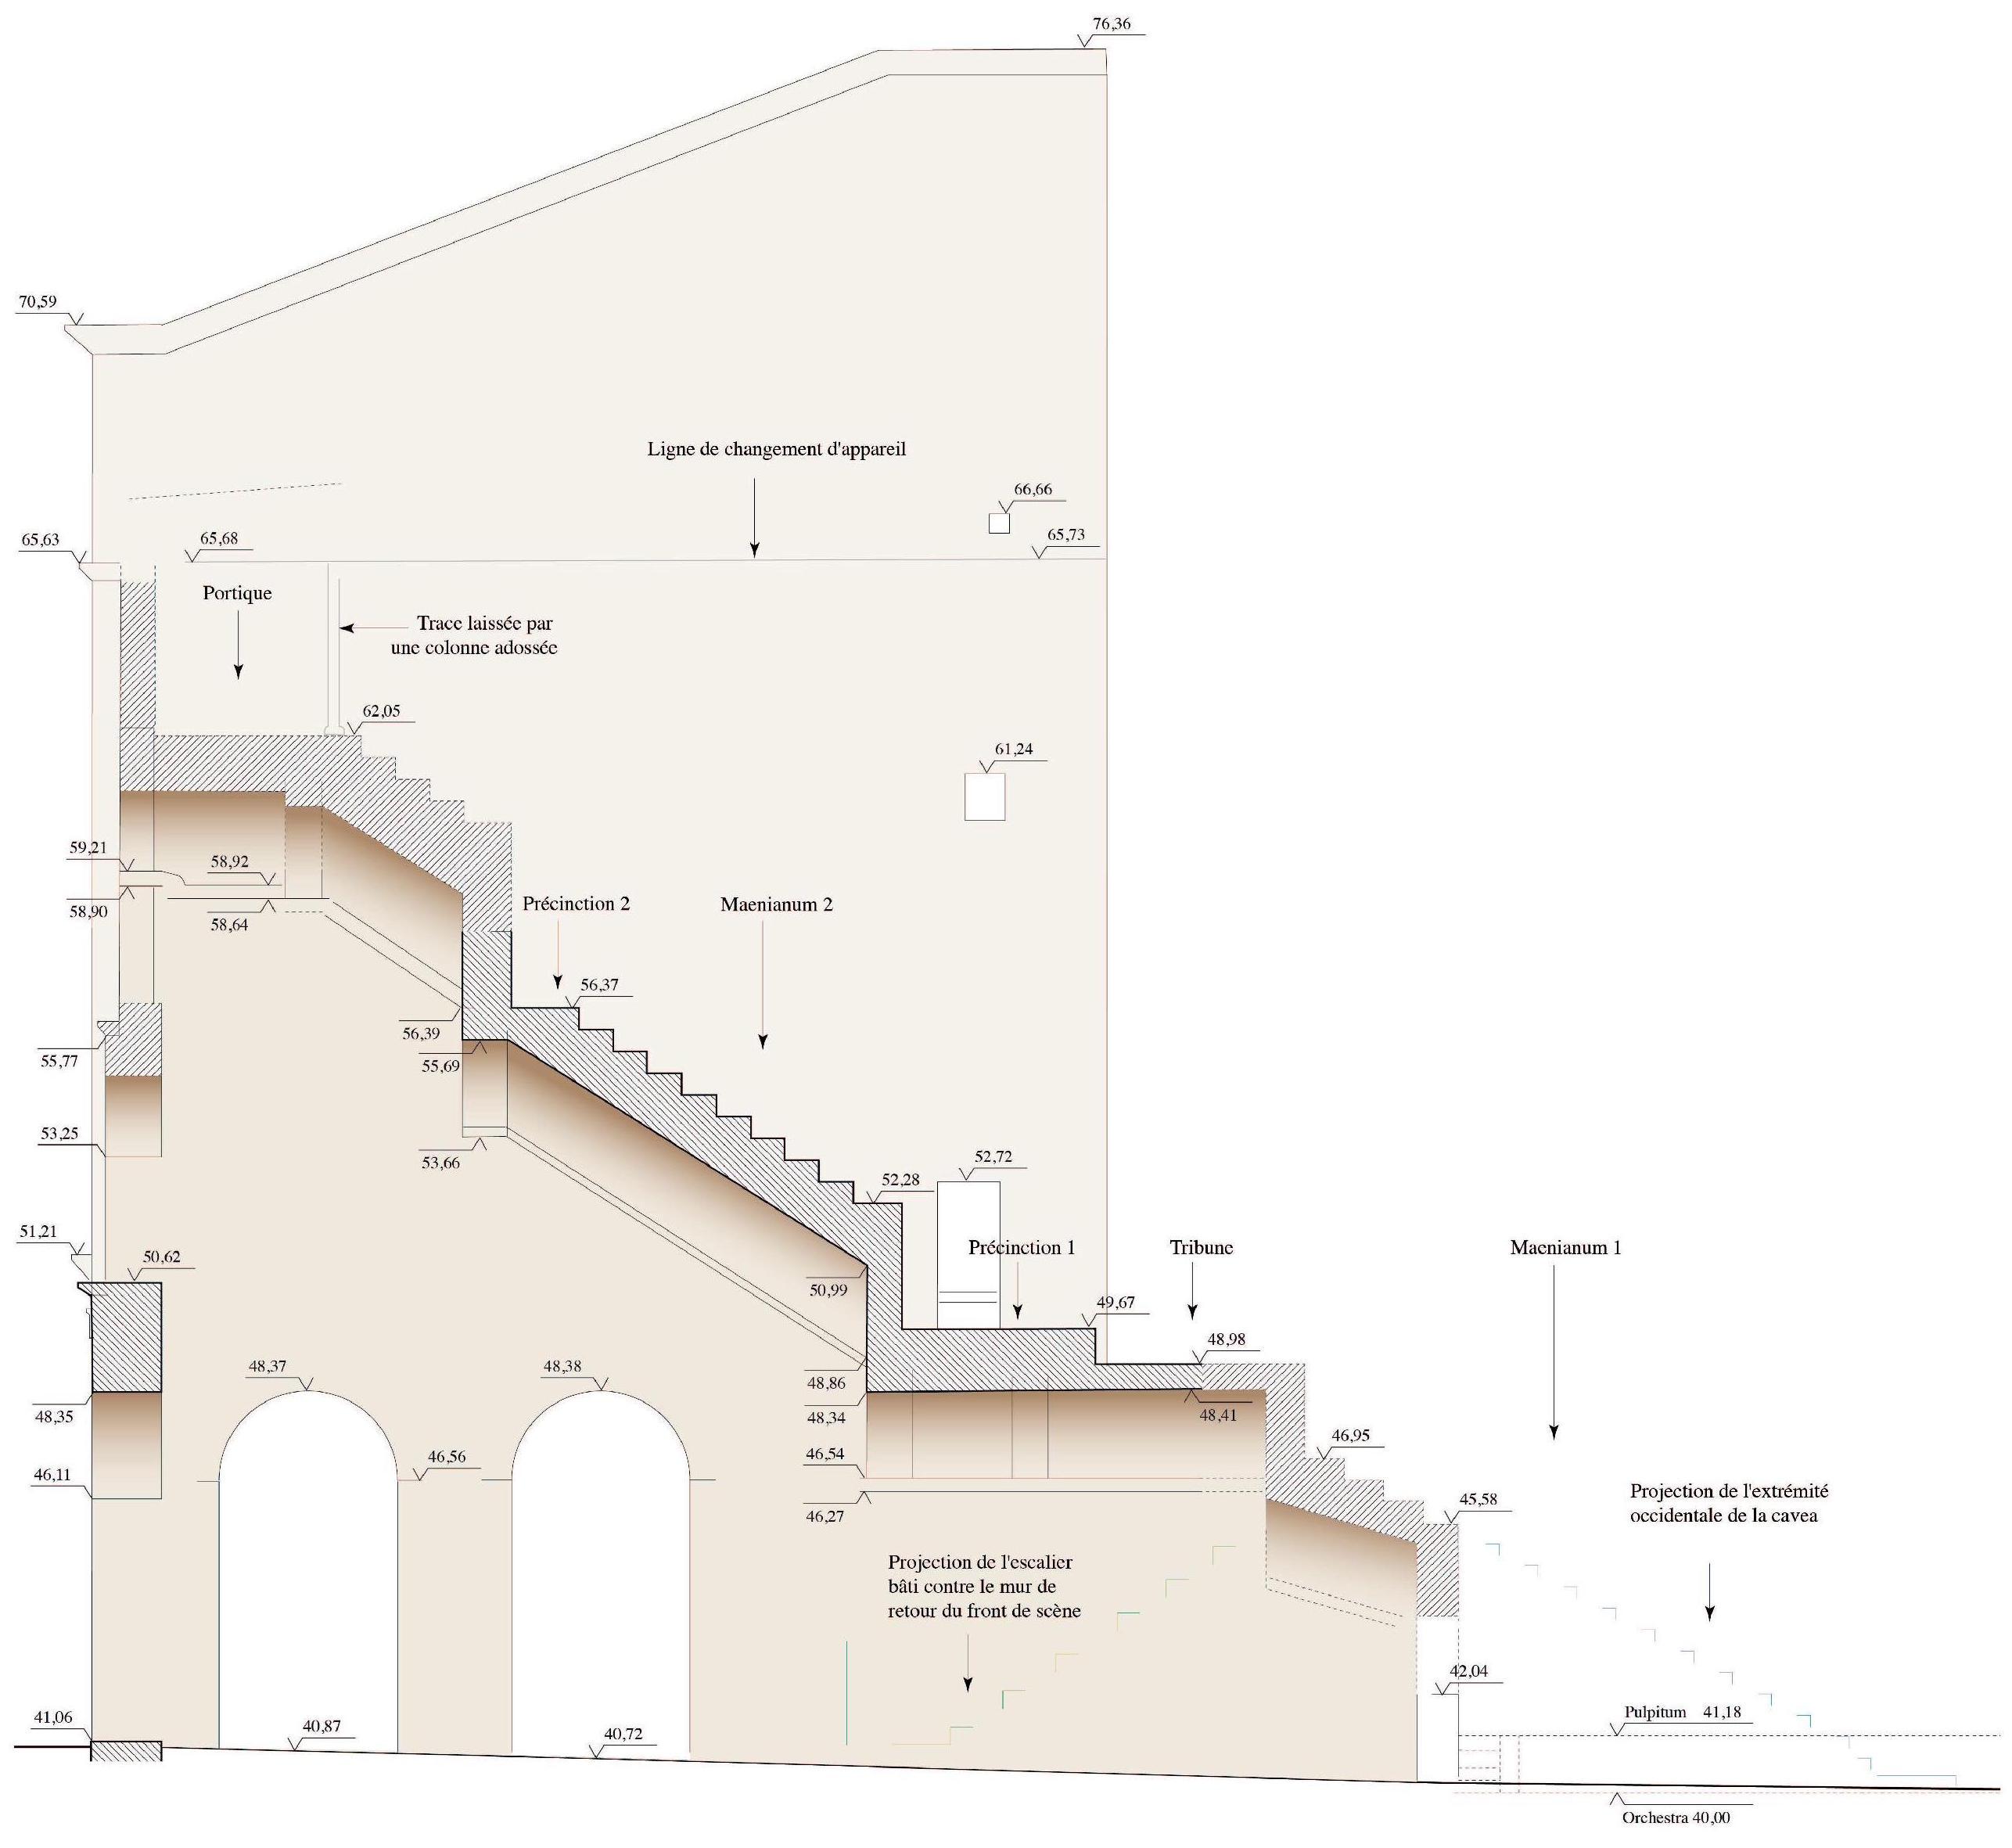
\includegraphics[width=\linewidth]{images/aditusOccidental}
		\caption[Coupe sur l'\gls{aditus} occidental]{Coupe sur l'\gls{aditus} occidental \cite[Pl. XLVIII]{orangePl}}
		\label{aditusOccidental}
	\end{subfigureth}	
	\begin{subfigureth}{0.49\textwidth}
		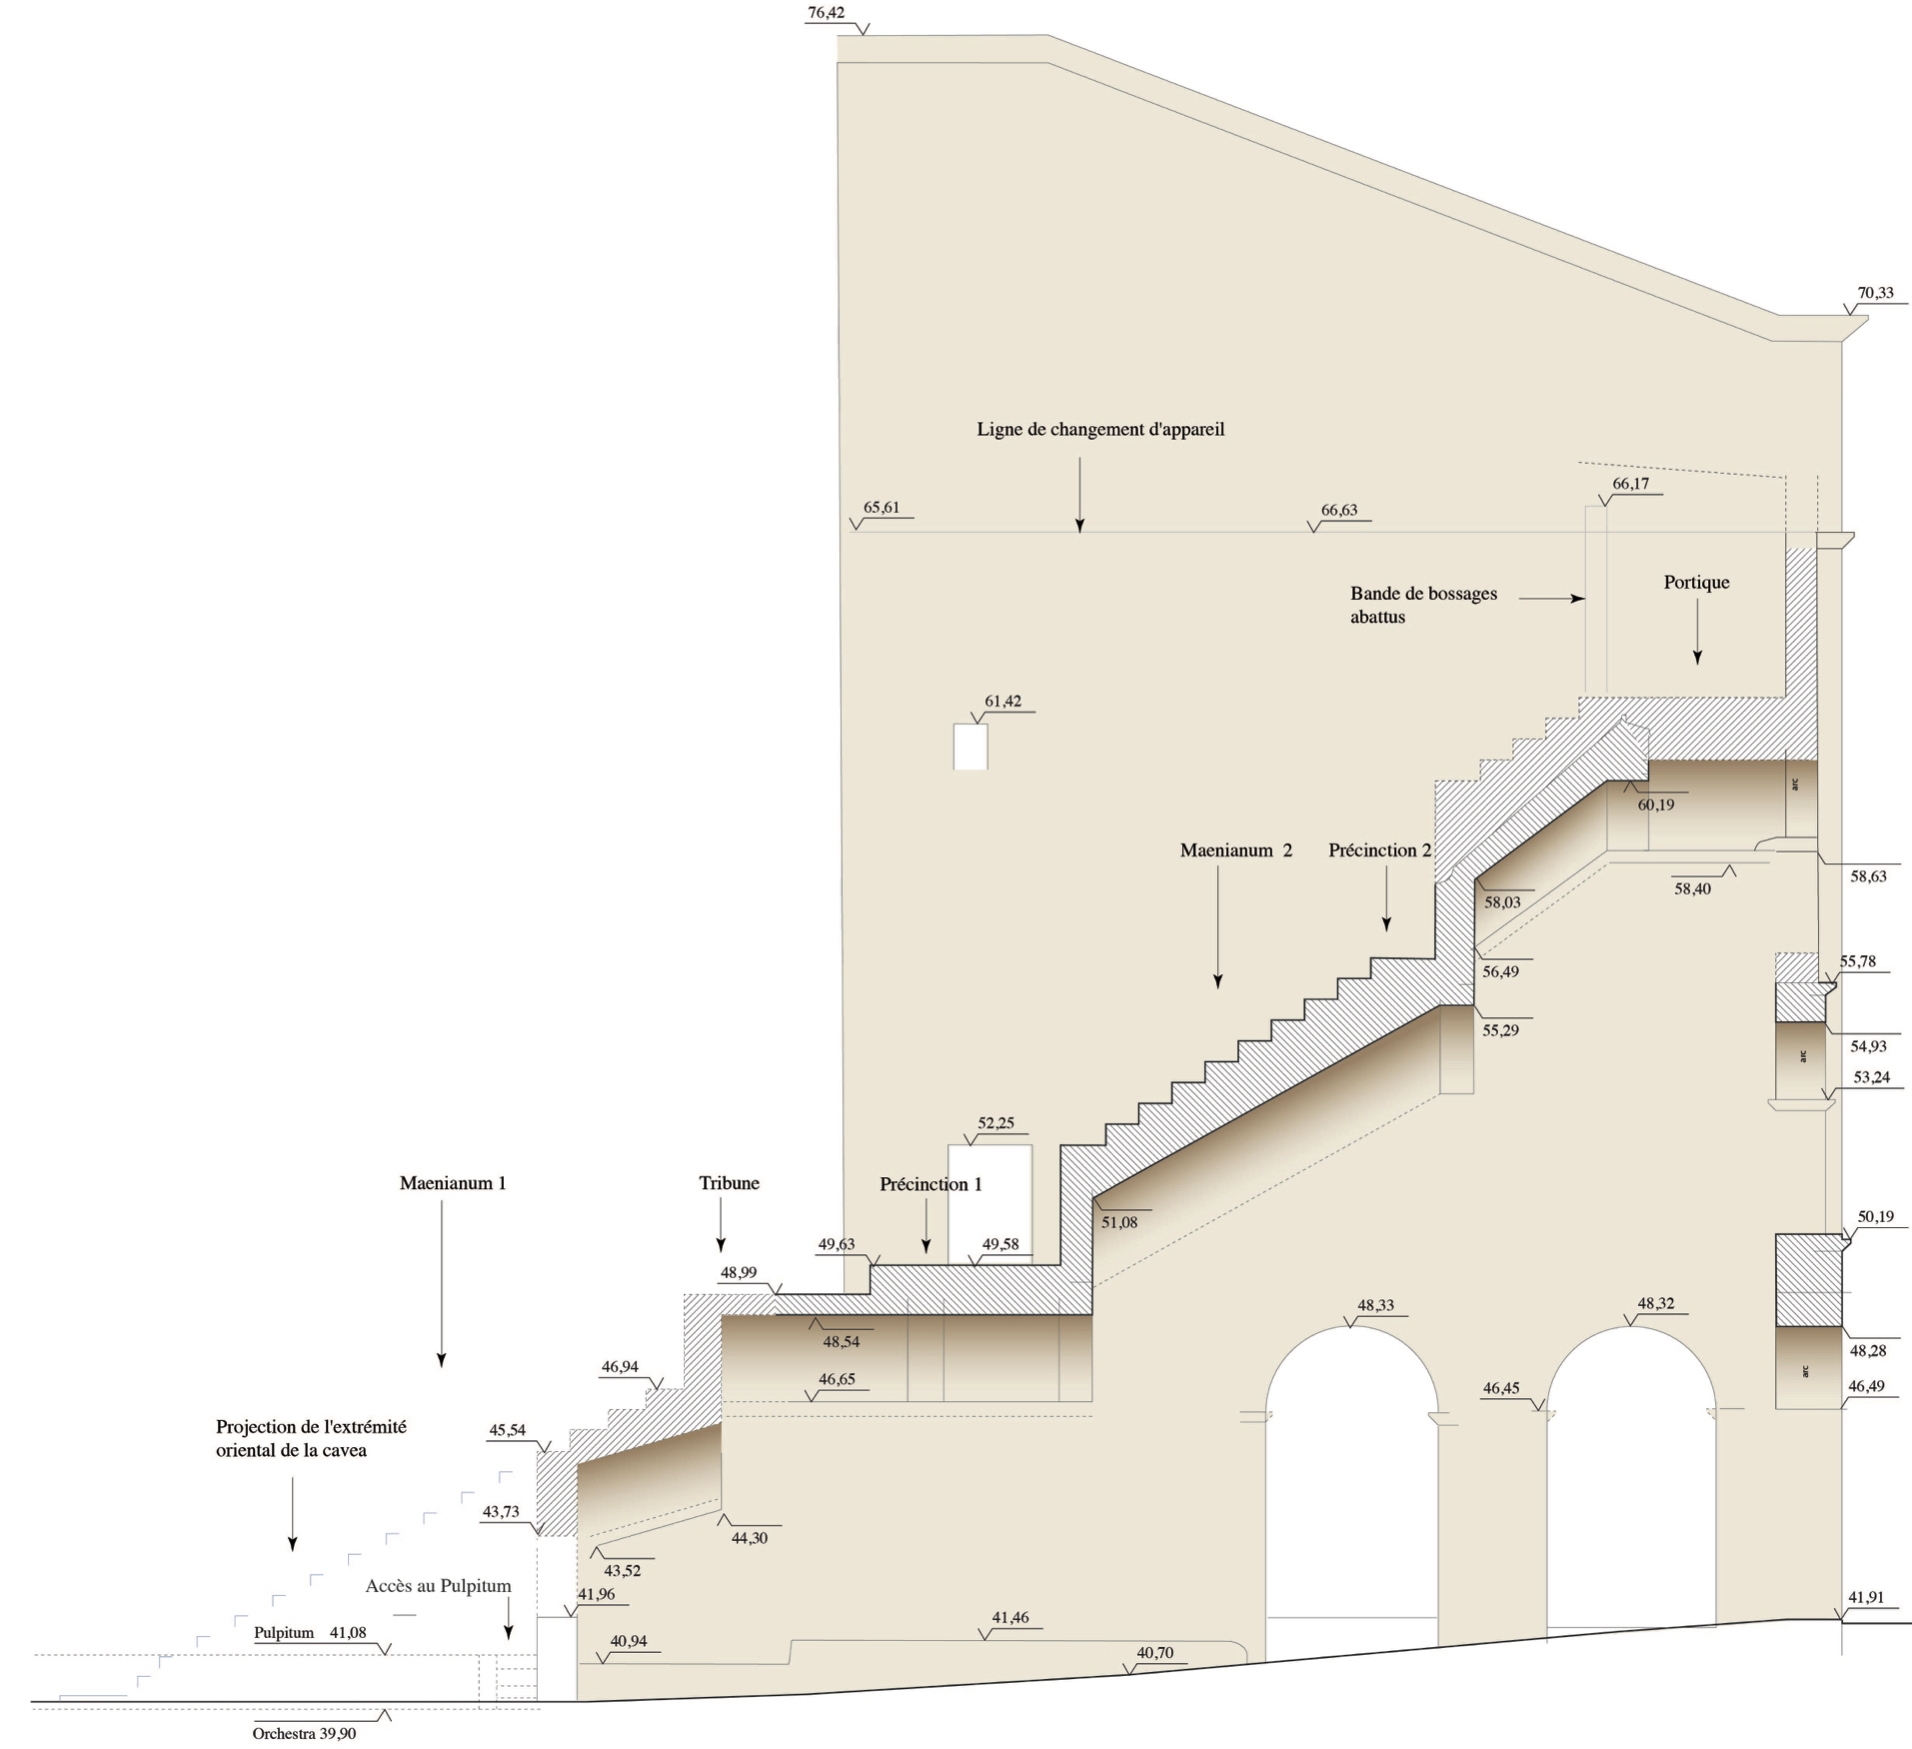
\includegraphics[width=\linewidth]{images/aditusOriental}
		\caption[Coupe sur l'\gls{aditus} oriental]{Coupe sur l'\gls{aditus} oriental \cite[Pl. XLIX]{orangePl}}
		\label{aditusOriental}
	\end{subfigureth}
	\label{aditus}
\end{figureth}

L'intérieur des aditus est composé d'un enchainement de voutes en berceau permettant le passage sous la cavea. Les mesures de ces voutes sont données par la figure \ref{aditusOccidental} pour l'aditus occidental et la figure \ref{aditusOriental} pour l'aditus oriental. Un objet à l'est et un objet à l'ouest épousant la forme de ces voutes sont créés par extrusions successives et est retirés des objets "aditus" par \gls{boolean}. Leur largeur est de 1,52m d'après \cite[Pl. XXI]{orangePl} et en appliquant le règle \ref{epaisseur}. Les aditus sont dans un premier temps symétrisés à l'identique à l'est et à l'ouest par recopie via un \gls{mirror}. Ils sont modélisés à partir de l'objet cavea que l'on coupe à partir du dizième gradin pour laisser l'espace aux \gls{parodos}. Le plan de coupe prend ensuite une épaisseur de 3,6m grâce à un \gls{solidify}. Il est important de noter que tant qu'un modifier n'est pas appliqué, il est toujours possible de le masquer ou de le modifier. A la différence du \gls{screw}, le \gls{solidify} permet l'utilisation du \gls{boolean} sans avoir besoin de l'appliquer définitivement. Cela laisse une grande flexibilité quand à la modifiabilité du modèle. Les aditus sont également percés par la porte (symétrisée en miroir) donnant accès au dixième gradins déjà évoquée à la section \ref{La cavea et ses substructures} ainsi que par deux grandes baies à arcature donnant dans les basiliques. Les figures \ref{aditusOccidental} et \ref{aditusOriental} en donne les élévations tandis que leur largeur est donnée par A.Caristie du coté occidental. Celles-ci seront réutilisée du coté oriental.

		\section{Le mur de scène et ses basiliques}

Le mur de scène ainsi que ses deux basiliques constituent un bloc distinct. La base est entièrement créée grâce aux cotes de la figure \ref{cotes}. La première étape est de tracé du segment de deux points aux coordonnées suivantes [-51,96 ; 21,92 ; 40] et [51,96 ; 21,92 ; 40] correspondant aux extrémités nord de la base du mur. On extrude alors ces points selon les axes X et Y afin de tracer la forme extérieure du mur. La seule partie qui n'est pas alignée sur l'un de ces deux axes est l'\gls{exedre} curviligne enclavant la porte royale. Celle-ci est modélisé à partir d'un cercle de 23,5m de diamètre pour lequel on ne garde que six segments à gauche et sept à droite qui forme la partie incurvée du mur. Une fois le contour de la base réalisé, le plan ainsi crée est extrudé verticalement jusqu'à 76,42m correspondant à la plus haute élévation du mur.
Sont ensuite crées des objets rectangulaires aux dimensions des pièces, et traversant le mur dans toute sa hauteur. A l'aide d'un \gls{boolean} ces objets sont soustraits à la forme de base. On note quelques valeurs aberrantes sur le plan de \cite[Pl. XXI]{orangePl} surement duent à des erreurs de recopie et qui sont à présent corrigées dans le modèle numérique. Lorsqu'une cote n'a pas été spécifiée, on considère la cote symétrique du mur. 

La même méthode est utilisée pour découper le haut du mur qui supportait le toit. On s'appuie alors sur la restitution de A.Caristie (voir figures \ref{toitCaristie} et \ref{toitBadie}) qui propose pour la partie sommitale du front de scène une taille en biseau permettant de soutenir les poutres allant des trous d'encastrement dans le mur nord à l'avant de la scène. On creuse donc également la façade sud du mur nord avec un objet de forme rectangulaire représentant une poutre basique et qui formera ces trous d'encastrement. Celle-ci est taillée pour entrer perpendiculairement dans le mur et on adopte le modèle générique \cite[Pl. XL]{orangePl}.
Ces poutres sont répétées à l'identiques à l'aide d'un \gls{array} car ces encastrements ont été détruit et recontruit par endroit ce qui rend la restitution très difficile (voir \cite[Pl. XXXVII]{orangePl}). Cela n'empêche pas les futurs améliorations par des archéologues experts dans une prochaine étape.

Pour réaliser les 17 portes donnant sur la \gls{porticus ps} on utilise également le plan \ref{cotes} en réalisant une mise à l'échelle lorsque les valeurs numériques de largeur ne sont pas indiquées. La modélisation de leurs élévations n'est malheureusement pas très précise car faute de valeur numérique, celles-ci sont estimées grâce aux dessins de H.Daumet \cite[Pl. XII, XIII, XIV]{orangePl}. Ce travail révèle que la porte royale n'est pas parfaitement centrée par rapport à la cavea mais est décalée de 32cm vers l'est. Ceci est peut-être dût à la façon dont a été conçu le modèle numérique et par la présence des nombreuses approximations stipulées plus haut. 

La façade du front de scène possède elle aussi des trous d'encastrement ayant pour leur part servis à accrocher la décoration. Ceux-ci sont créés à l'aide d'un \gls{boolean} en respectant les mesures d'élévation de \cite[Pl. XXIX]{orangePl}. Sur cette même façade sont également percées les trois portes traversant le \gls{postscaenium} ainsi que différents autres encastrement. Tous sont modélisés par mise à l'échelle des plans de \cite{orangePl} et sont symétrisés par rapport à la porte royale. De part et d'autre de celle-ci se trouvent deux niches créées par la soustraction d'un demi-cylindre verticale. Au-dessus, à la frontière avec le second ordre se trouvent de petites baies à arcature. Encore au dessus et centré sur le front de scène se trouve une grande niche abritant aujourd'hui une statue dite d'Auguste. Cette niche est l'emprunte d'un demi-cylindre vertical dont la face supérieur est un demi-cylindre horizontal.


		\section{Le pulpitum et l'orchestra} 

Le pultpitum, autrement dit l'estrade de scène a complètement disparu et a aujourd'hui été remplacé par un plancher moderne. Il reste néanmoins des traces sur le mur de scène qui permettent de le modéliser dans sa version antique. Les planches XLVII et XLIX \cite{orangePl} donnent les élévations du pulpitum ainsi que de l'orchestre sure les extrémités orientales et occidentales. L'orchestre est une forme volumique dont la face supérieure représente le sol. Il sera dans une prochaine étape creusé à l'aide de modifiers Boolean pour l'hyposcaenium et le caniveau décrit dans une autre partie.

		\section{La colline Saint-Eutrope} 
Comme souvent les architectes de l'époque ont adossé la cavea sur un relief naturel afin de solidifier la structure et de simplifier la construction de l'édifice. La colline Saint-Eurtope qui soutient donc le théâtre sur sa partie méridionale a été modélisée d'après les lignes d'altitude (fig. \ref{colline}) à partir de la plus basse jusqu'à la plus haute par pas de 6m par extrusion successive. Les élévation ont ensuite été légèrement adaptée (ligne par ligne) pour s'encastrer au mieux dans le théâtre. La colline est donc actuellement peu précise et il est nécessaire de l'affiner à l'aide d'un document détaillant mieux sa géométrie.

\begin{figure}[!h]
	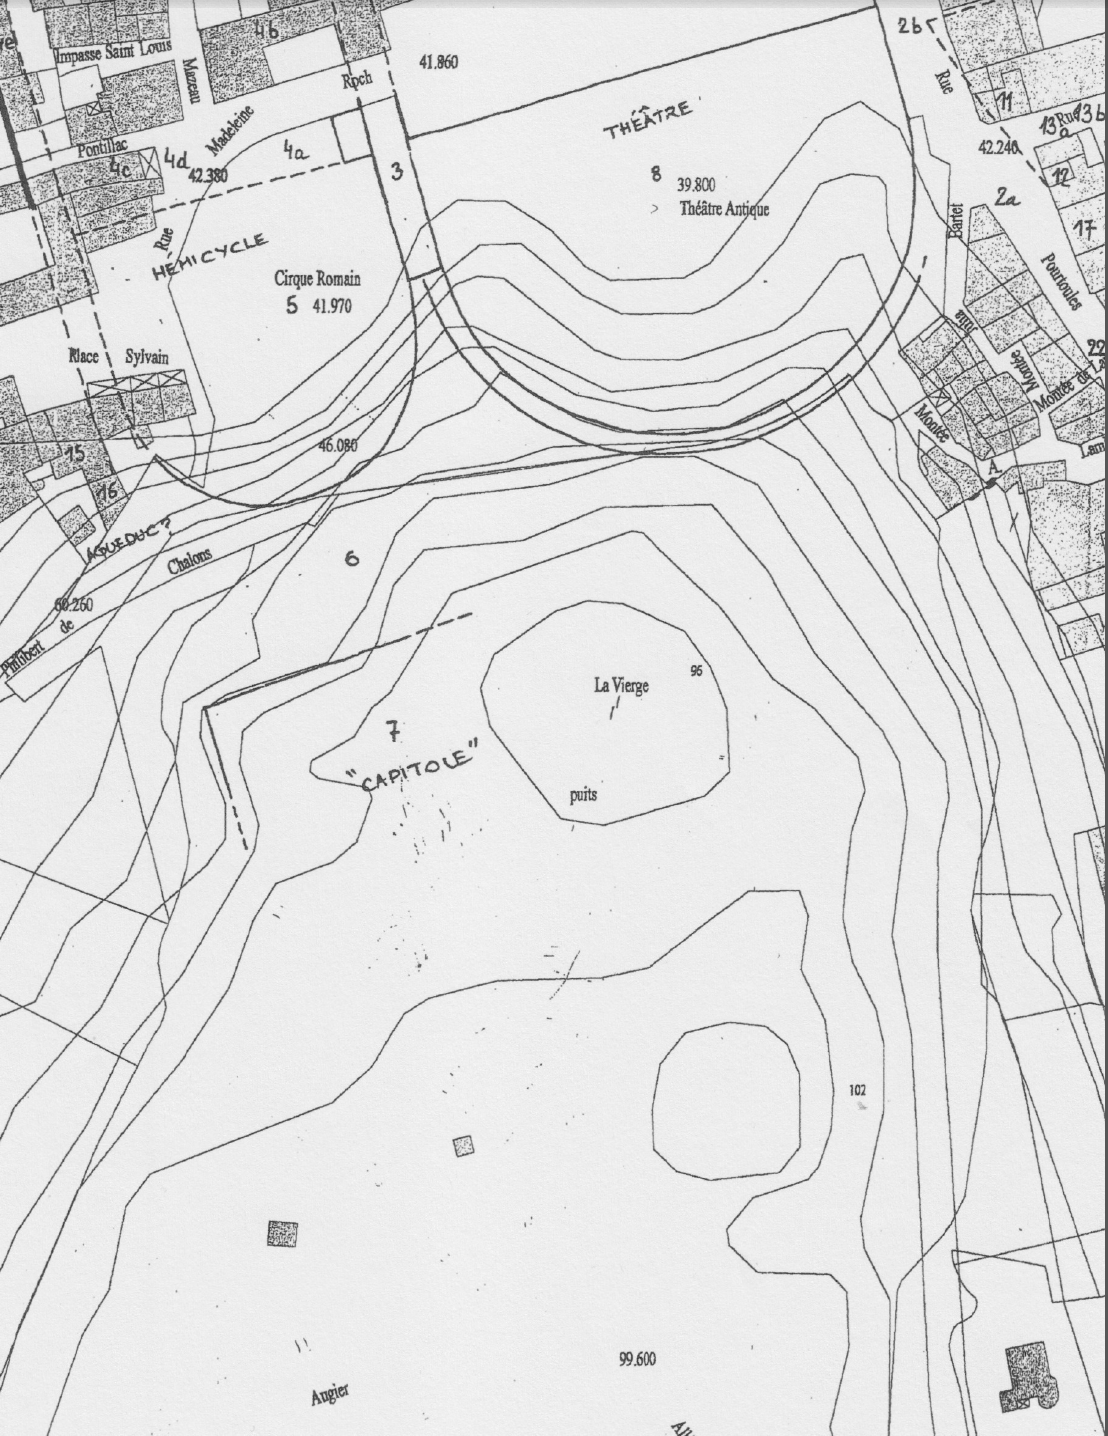
\includegraphics[width=\linewidth]{images/colline}
	\caption[Plan topographique de la colline Saint-Eutrope]{Plan topographique de la colline Saint-Eutrope \cite[p.11]{orangeTxt}}
	\label{colline} 
\end{figure} 


		
	\chapter{Propositions de reconstitution}
		\citationChap{
		Imagination is as effortless as perception, unless we think it might be ‘wrong’, which is what our education encourages us to believe.
		}{Keith Johnstone}
		\minitoc
		\newpage
		
	\chapter*{Conclusion}
	\addcontentsline{toc}{chapter}{Conclusion}
		\newpage
			
% Biblio
%\titleformat{\chapter}[hang]{\bf\huge}{}{2pc}{} % Pour enlever "Chapitre N"
 %\titleformat{\chapter}[display]{\bf\huge}{Chapitre \thechapter}{2pc}{} % Pour remettre "Chapitre N"
 \bibliographystyle{francaissc}
 \bibliography{Part1/Biblio}
\addcontentsline{toc}{chapter}{Références}


